\documentclass[xcolor=dvipsnames]{beamer}

% 1. PREÁMBULO: Configuraciones Globales
\usetheme{Madrid}
\usepackage[utf8]{inputenc}
\usepackage[spanish, es-tabla]{babel} % es-tabla para que diga Tabla y no Cuadro
\usepackage{amsmath, amssymb}
\usepackage{diagbox}
\usepackage{multirow}
\usepackage{tikz}

% 2. CONFIGURACIÓN DE TIKZ (Debe ir en el preámbulo)
\usetikzlibrary{arrows.meta, positioning, calc}
\tikzset{
    state/.style={circle, draw=black, thick, minimum size=1.1cm, font=\bfseries},
    alc/.style={state, fill=Emerald!20, text=Emerald!70!black},
    baj/.style={state, fill=Maroon!20, text=Maroon!70!black},
    est/.style={state, fill=Gray!20, text=Gray!70!black},
    trans/.style={->, >={Stealth[scale=1.0]}, thick, black!70, shorten >=1pt},
    val/.style={font=\tiny\bfseries, text=blue!80!black, yshift=2mm}
}

\title{Toma de Decisiones Secuenciales \\ y Aprendizaje por Refuerzo}
\author{Daniela Pucci de Farias}
\institute{Universidad Torcuato Di Tella}
\date{Modulo 2: MDPs}

% 3. PERSONALIZACIÓN DEL FOOTER (Muestra únicamente: Módulo | Páginas con margen izquierdo)
\setbeamertemplate{footline}{
  \leavevmode%
  \hbox{%
  % Bloque 1 (Izquierda/Centro): Nombre del Módulo con más espacio al borde (leftskip)
  \begin{beamercolorbox}[wd=.8\paperwidth,ht=2.25ex,dp=1ex,leftskip=4ex,left]{title in head/foot}%
    \usebeamerfont{title in head/foot}\hspace*{2ex} \insertdate
  \end{beamercolorbox}%
  % Bloque 2 (Derecha): Numeración de Páginas
  \begin{beamercolorbox}[wd=.2\paperwidth,ht=2.25ex,dp=1ex,right]{date in head/foot}%
    \usebeamerfont{date in head/foot}
    \insertframenumber{} / \inserttotalframenumber\hspace*{2ex} 
  \end{beamercolorbox}}%
  \vbox{}%
}


\begin{document}

\frame{\titlepage}
% --- SLIDE: REPASO RÁPIDO DEL MRP ---
\begin{frame}{Recapitulando: El Proceso de Recompensa (MRP)}
En la \'ultima clase, exploramos el marco de MRPs para modelar la evoluci\'on de sistemas bajo incertidumbre. MRPs se caracterizan por la tupla $(S, P, R)$:

\begin{itemize}
    \item \textbf{Estado ($S$):} Representaci\'on compacta del presente.
    \item \textbf{Transici\'on ($P$):} Probabilidad pasiva de cambio ($s \to s'$).
    \item \textbf{Recompensa ($R$):} Valor asociado a cada estado visitado.
\end{itemize}

\only<2->{
\begin{block}{Funci\'on Valor}
   Uno de los conceptos centrales en MRP es el de la funci\'on valor $V_t(s)$, que captura el valor esperado presente y futuro de estar en un cierto estado, en un cierto momento en el tiempo.
\end{block}}

\only<3->{
En el contexto de MRPs, la funci\'on valor nos permite evaluar, por ejemplo, reglas fijas que usamos para tomar decisiones, como las estrat\'egias de control de stock que vimos.}
\end{frame}

% --- SLIDE: MDP (VERSIÓN MEJORADA) ---
\begin{frame}{Procesos Markovianos de Decisi\'on (MDP)}
El MDP introduce la capacidad de afectar el ambiente mediante acciones.

\begin{center}
    % Aquí puedes mantener tu imagen RL3.png o usar un diagrama de flujo Agente-Entorno
    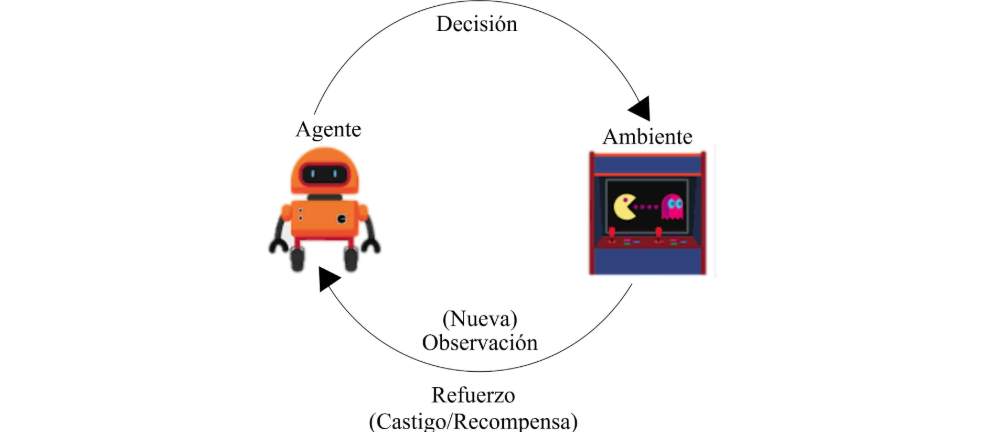
\includegraphics[width=0.5\textwidth]{../Images/Figures/RL3.png}
\end{center}

\begin{itemize}
    \item<2-> \textbf{Acciones ($A$):} El conjunto de decisiones disponibles en cada estado.
    \item<3-> \textbf{Transiciones Din\'amicas $P_a(s,s')$}:
    \begin{itemize}
        \item El azar sigue existiendo, pero la acci\'on $a$ afecta transiciones.
    \end{itemize}
    \item<4-> \textbf{Recompensa $r_a(s)$:} 
    \begin{itemize}
        \item El beneficio ya no depende solo de d\'onde estamos, sino de tambi\'en \textbf{qu\'e hacemos} en ese momento.
    \end{itemize}
\end{itemize}

\uncover<5->{
    \begin{alertblock}{Definici\'on Formal}
        Un MDP es la tupla $(S, A, P, r)$ que modela el ciclo interactivo de decisi\'on.
    \end{alertblock}
}
\end{frame}


% --- SLIDE: DISCUSIÓN ---

\begin{frame}{Discusión: Eres el Gerente de una Aerolínea}

\textbf{Escenario:} Entra una solicitud de reserva.

\begin{itemize}
\item \textbf{Opción A:} Cobrar \$50 (venta casi segura).
\item \textbf{Opción B:} Cobrar \$120 (mayor margen, pero riesgo de no vender).
\end{itemize}

\vspace{0.4cm}

\begin{block}{¿Qué harías tú?}
\begin{itemize}
\item ¿Qué información considerarías para decidir?
\item ¿Cómo cambia tu decisión si falta 1 día vs. 30 días para el vuelo?
\item ¿Existe una regla simple que funcione siempre?
\end{itemize}
\end{block}

\end{frame}

% --- SLIDE: HEURÍSTICAS ---

\begin{frame}{Antes del Revenue Management Moderno}

Históricamente, muchas decisiones de precios se tomaban mediante reglas simples y experiencia acumulada.

\begin{itemize}
\item \textbf{Precios por segmentos fijos:}
Turista \$70, Primera Clase \$200.

\item \textbf{Heurísticas de ocupación:}
\begin{itemize}
    \item Si el avión está al 50\% un mes antes, subir el precio.
    \item Si falta una semana y sobran asientos, hacer descuentos.
\end{itemize}

\item \textbf{Costo más margen:}
Calcular el costo del asiento y agregar un porcentaje fijo.

\end{itemize}

\vspace{0.3cm}

\textit{Estas reglas suelen capturar parte de la intuición del problema, pero no cuantifican explícitamente el valor futuro de un asiento disponible.}

\end{frame}

% --- SLIDE: LIMITACIONES ---

\begin{frame}{¿Cuáles son las limitaciones de las heurísticas?}

Aunque suelen ser intuitivas y fáciles de implementar, las reglas fijas presentan algunas limitaciones:

\begin{itemize}
\item \textbf{Rigidez:} Pueden reaccionar mal ante cambios inesperados en la demanda.
\item \textbf{Miopía:} No cuantifican adecuadamente el impacto de las decisiones actuales sobre oportunidades futuras.

\item \textbf{Inconsistencia:} Distintos tomadores de decisión pueden llegar a conclusiones diferentes usando la misma información.


\end{itemize}

\vspace{0.3cm}

\begin{alertblock}{¿Qué necesitamos?}
Para mejorar estas decisiones necesitamos:

\begin{enumerate}
\item Un modelo de la incertidumbre del mercado.
\item Una forma de cuantificar el valor de las oportunidades futuras.
\end{enumerate}
\end{alertblock}

\end{frame}

% --- SLIDE: INGREDIENTE 1 ---

\begin{frame}{Ingrediente 1: Modelar la Incertidumbre}

Para tomar decisiones racionales necesitamos un modelo de la demanda.

A partir de datos históricos y segmentación de clientes, la aerolínea estima cómo se distribuye la disposición a pagar de los pasajeros.

\vspace{0.2cm}

Cada día llega un cliente potencial con una disposición a pagar máxima $m$.

La aerolínea no conoce el valor de $m$ para cada cliente, pero sí su distribución:

\begin{itemize}
\item $P(m = 50)=1/2$
\item $P(m = 70)=1/3$
\item $P(m = 120)=1/6$
\end{itemize}

\textquestiondown ¿Cómo interpretarías esta distribución?

\vspace{0.2cm}

\textit{Este modelo captura la incertidumbre del mercado.}

\end{frame}


% --- SLIDE: INGREDIENTE 2 ---

\begin{frame}{Ingrediente 2: Cuantificar el Valor Futuro}

Necesitamos cuantificar el impacto futuro de una decisión tomada hoy.

\vspace{0.2cm}

\begin{itemize}
\item ¿Cuánto vale realmente un asiento libre?
\item ¿Cómo influye ese valor en el precio que deberíamos ofrecer?
\end{itemize}


\only<2->{
Idea: Asignamos un valor a cada estado. Ese valor resume todas las recompensas futuras que esperamos obtener desde allí.
}

\only<3->{
\begin{block}{Regla de Decisión}
Elegimos la acción $a$ que maximiza:
\[
\underbrace{r_a(s)}_{\text{Beneficio inmediato}}
+
\underbrace{\mathbb{E}[V_{t-1}(s')|s,a]}_{\text{Valor de las oportunidades futuras}}
\]
\end{block}

\vspace{0.3cm}

\textit{$V_{t-1}(s')$ resume todo lo que esperamos ganar desde el próximo período hasta el final del horizonte si seguimos actuando de manera óptima.}
}

\end{frame}




\begin{frame}{Ejemplo: Precios Dinámicos - Modelo MDP - $(S,A,P,r)$}

Un vuelo tiene capacidad para 100 pasajeros. Cada d\'ia llega un cliente potencial con disposici\'on a pagar un precio m\'aximo $m$.

\textbf{Incertidumbre del Mercado:}
La aerol\'inea desconoce $m$, pero conoce su distribuci\'on:
\begin{itemize}
    \item $P(m = 50) = 1/2$,  $P(m = 70) = 1/3$, $P(m = 120) = 1/6$.
\end{itemize}
\begin{center}
\visible<2->{
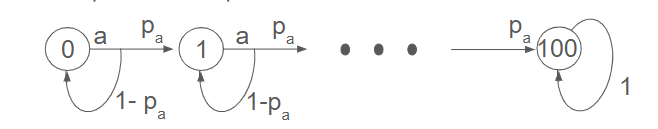
\includegraphics[width=0.9\textwidth]{../Images/Figures/Airline.png}
\begin{tabular}{|c|c|c|}
\hline
$a$ & $P_a(x,x+1) = {\rm Prob}(m\geq a) = p_a$ & $r_a(x) = a p_a$\\
\hline
50 & 1 & 50 \\
\hline
70 & 0.5 & 35 \\
\hline
120 & 1/6 & 20 \\
\hline
\end{tabular}}
\end{center}
\end{frame}

\begin{frame}{Ejemplo: Precios Dinámicos - Modelo MDP - $(S,A,P,r)$}

Formalizando:
\begin{itemize}
\item<2-> {\bf Espacio de estados $S = \{0,1,\dots,100\}$}
\item<3-> {\bf Espacio de acciones $A = \{50, 70, 120\}$}
\item<4-> {\bf Matriz de transición P} 
$$
\begin{array}{ccl}
P_a(100,100) & = & 1, ~\forall a \in A \\
P_a(x,x+1) & = & {\rm Prob}(m\geq a) \equiv p_a,~\forall x<100,~a \in A \\
P_a(x,x) & = & {\rm Prob}(m<a) \equiv 1-p_a,~\forall x<100,~a \in A  
\end{array}
$$

\item<5-> {\bf Recompensa r} 
$$
\begin{array}{ccl}
r_a(x) &=& a p_a,~\forall x=0,\dots,99,~a \in A\\
r_a(100) & = & 0,~\forall a \in A
\end{array}
$$
\end{itemize}
\end{frame}



%% --- SLIDE: EL FACTOR TIEMPO - HORIZONTE DE DECISIÓN ---
%\begin{frame}{El Factor Tiempo: ¿Cuándo termina el juego?}
%En Revenue Management, el inventario es perecedero. El valor de un asiento cae a cero en el momento en que el avión despega.
%
%\begin{itemize}
%    \item \textbf{Horizonte Finito ($T$):}
%    \begin{itemize}
%        \item Existe un d\'ia final para el proceso (fecha del vuelo).
%        \item La estrategia es inherentemente no estacionaria: el precio óptimo depende de cuántos días faltan.
%\begin{itemize}
%\item Si quedan 10 asientos y faltan 100 d\'ias, ¿ofreces el precio de 50 o el de 120? ¿Y si falta solo 1 d\'ia?
%\end{itemize}
%    \end{itemize}
%    
%    \item \textbf{El Estado Aumentado:}
%    \begin{itemize}
%        \item ¿Basta con saber la ocupación $x$? 
%        \item No. El estado real debe ser la tupla $(x, t)$, donde $t$ es el tiempo restante. 
%\begin{itemize}
%\item Pero el tiempo es una variable de estado especial, en el marco de MDPs podemos considerarla separadamente ($V_t(s)$).
%\end{itemize}
%    \end{itemize}
%\end{itemize}
%
%\end{frame}

\begin{frame}{Decidiendo con la Funci\'on Valor}
\begin{block}{Regla de Decisión Intuitiva}
    Elegimos la acción $a$ que maximiza:
    \[ \underbrace{r_a(s)}_{\text{Presente}} + \underbrace{\mathbb{E}[V_{t-1}(s')]}_{\text{Futuro Prometido}} \]
\end{block}
\begin{itemize}
\item Si conocemos a la funci\'on valor, esa puede ser una buena manera de decidir (de hecho, es \'optima).
\item \textquestiondown C\'omo calcularla?
\end{itemize}
\end{frame}

% --- SLIDE 3: CÁLCULO PASO A PASO CON GRAFO ---
\begin{frame}{Recordamos la Recursi\'on para MRPs...}

\tikzset{
    state_bw/.style={circle, draw=black, thick, minimum size=0.9cm, font=\bfseries},
    trans/.style={->, >={Stealth[scale=1.0]}, thick, black!70, shorten >=1pt},
    val_label/.style={font=\tiny\bfseries, text=blue!80!black, yshift=2mm}
}

\centering

% 1. ECUACIÓN SUPERIOR: EL MODELO GENERAL
\small
\begin{itemize}
    \item[] \textbf{Caso Base ($t=0$):} $V_0(s) = r(s)$ 
    \item<2->[] \textbf{Paso de Inducción ($t>0$):} $V_t(s) = r(s) + \sum_{s'} P(s,s')V_{t-1}(s')$
\end{itemize}

\vspace{0.2cm}

\begin{tikzpicture}[node distance=1.8cm, scale=0.85, every node/.style={scale=0.85}]
    % Nodos de tiempo
    \node (t0) at (0, 3.2) {\textbf{Hoy} ($t=2$)};
    \node (t1) at (3.5, 3.2) {\textbf{Semana 1} ($t=1$)};
    \node (t2) at (7, 3.2) {\textbf{Semana 2} ($t=0$)};
    
    % Columna t=2
    \node[state_bw] (A0) at (0, 2) {A};
    \node[state_bw] (B0) at (0, 0.5) {B};
    \node[state_bw] (E0) at (0,-1) {E};
    
    % Columna t=1
    \node[state_bw] (A1) at (3.5, 2) {A};
    \node[state_bw] (B1) at (3.5, 0.5) {B};
    \node[state_bw] (E1) at (3.5,-1) {E};

    % Columna t=0 (Caso Base)
    \node[state_bw] (A2) at (7, 2) {A};
    \node[state_bw] (B2) at (7, 0.5) {B};
    \node[state_bw] (E2) at (7,-1) {E};

    % VALORES CASO BASE
    \node[val_label] at (A2.north) {$V_0(A)=0.005$};
    \node[val_label] at (B2.north) {$V_0(B)=-0.005$};
    \node[val_label] at (E2.north) {$V_0(E)=0$};

    % INDICACIÓN DE REPETICIÓN - Agregado punto y coma final si faltaba en algún bloque
    \draw[trans, thin] (A1) -- (A2);
    \draw[trans, thin] (A1) -- (B2);
    \draw[trans, thin] (A1) -- (E2); 
    \draw[trans, thin] (B1) -- (A2);
    \draw[trans, thin] (B1) -- (B2);
    \draw[trans, thin] (B1) -- (E2); 
    \draw[trans, thin] (E1) -- (A2);
    \draw[trans, thin] (E1) -- (B2);
    \draw[trans, thin] (E1) -- (E2); 
    \draw[trans, thin] (A0) -- (A1);
    \draw[trans, thin] (A0) -- (B1);
    \draw[trans, thin] (A0) -- (E1); 
    \draw[trans, thin] (B0) -- (A1);
    \draw[trans, thin] (B0) -- (B1);
    \draw[trans, thin] (B0) -- (E1); 
    \draw[trans, thin] (E0) -- (A1);
    \draw[trans, thin] (E0) -- (B1);
    \draw[trans, thin] (E0) -- (E1); 

    % CÁLCULO DE V1(A)
    \draw<2->[trans, blue, thin] (A1) -- (A2) node[midway, above, font=\tiny] {0.9};
    \draw<2->[trans, blue!50, thin] (A1) -- (B2) node[pos=0.7, above, font=\tiny] {0.075};
    \draw<2->[trans, blue!50, thin] (A1) -- (E2) node[pos=0.8, swap, above, font=\tiny] {0.025};
    
\end{tikzpicture}

\vspace{0.3cm}
\begin{itemize}
\item<3->[] \textbf{Ahora vamos a hacer lo mismo, pero para MDPs.}
\end{itemize}

\end{frame}

% --- SLIDE: INDUCCIÓN HACIA ATRÁS - CASO BASE ---
\begin{frame}{Inducción Hacia Atrás: El Final del Horizonte}
Sea $V_t(s)$ el valor máximo esperado faltando $t$ días para el vuelo con $s$ asientos ocupados.

\textbf{Paso 1: Caso Base ($t=0$)}
En el momento del despegue, no hay más oportunidades de venta.

\begin{itemize}
    \item Si el avión despega, el valor de los asientos libres es nulo.
    \item $V_0(s) = \max_a r_a(s)$ para todo $s \in \{0, \dots, 100\}$.
\end{itemize}

\begin{center}
\begin{tikzpicture}[node distance=2cm]
    \node[circle, draw, thick, minimum size=1.2cm] (s) {$s$};
    \node[above=0.2cm of s, blue] {$V_0(s) = \max_a r_a(s)$};
    \node[right=2cm of s] (fin) {\textbf{Despegue}};
    \draw[->, thick] (s) -- (fin);
\end{tikzpicture}
\end{center}

\textit{Nota: En $t=0$, el futuro no importa. Tomamos la acci\'on que maximice la recompensa inmediata.}
\end{frame}

% --- SLIDE: INDUCCIÓN HACIA ATRÁS - PASO t=1 (CORREGIDO) ---
\begin{frame}{Inducción Hacia Atrás: El Salto a $t=1$}
\tikzset{
    % Estilo de nodos con tamaño fijo y centrado
    state_bw/.style={circle, draw=black, thick, minimum size=1.0cm, text width=0.8cm, align=center, font=\bfseries},
    trans/.style={->, >={Stealth[scale=1.0]}, thick, black!70, shorten >=1pt},
    % Estilo de etiqueta: ahora posicionado a la derecha
    val_label/.style={font=\small\bfseries, text=blue!80!black, xshift=2mm}
}

Faltando 1 d\'ia ($t=1$), si tenemos $s$ ocupados y ofrecemos el precio $a$:

\begin{itemize}
    \item \textbf{Venta ($p_a$):} Ganamos $a$ y pasamos a $s+1$ en $t=0$.
    \item \textbf{No Venta ($1-p_a$):} No ganamos nada y seguimos en $s$ en $t=0$.
\end{itemize}

\centering
\vspace{0.2cm}
\begin{tikzpicture}[scale=0.9]
    % Nodos de tiempo
    \node (t0) at (0, 3.5) {$t=1$};
    \node (t1) at (5, 3.5) {$t=0$ (despegue)};
    
    % Columna t=1
    \node[state_bw] (s_actual) at (0, 1.25) {s};
    
    % Columna t=0
    \node[state_bw] (s0) at (5, 2.2) {s};
    \node[state_bw] (s10) at (5, 0.3) {s+1};

    % VALORES CASO BASE (Posicionados a la derecha de los nodos)
    \node[val_label, anchor=west] at (s0.east) {$V_0(s)$};
    \node[val_label, anchor=west] at (s10.east) {$V_0(s+1)$};

    % TRANSICIONES
    \draw[trans] (s_actual) -- (s0) node[midway, sloped, above, font=\tiny] {$1-p_a$};
    \draw[trans] (s_actual) -- (s10) node[midway, sloped, below, font=\tiny] {$p_a$};
\end{tikzpicture}

\vspace{0.1cm}
\only<2->{
\textbf{Valor de la acci\'on $a$ en el estado $s$:}
\[
\begin{aligned}
Q_1(s, a) &= p_a [ a + V_0(s+1) ] + (1-p_a) [ V_0(s) ] \\
 &= \underbrace{a p_a}_{r_a(s)} + \sum_{s' \in \{s, s+1\}} P_a(s, s') V_0(s')
\end{aligned}
\]
}
\end{frame}

% --- SLIDE: LA ECUACIÓN DE BELLMAN ---
\begin{frame}{La Ecuaci\'on de Bellman: Optimizaci\'on General}
Para encontrar el valor m\'aximo en $t=1$, elegimos el precio que maximiza la suma de la recompensa inmediata y el valor futuro:
$$
V_1(s) = \max_{a \in A} \left\{ r_a(s) + \sum_{s'} P_a(s,s')V_0(s') \right\} 
$$

\textbf{Generalizando para cualquier d\'ia $t$:}

\begin{alertblock}{Ecuaci\'on de Bellman (Horizonte Finito)}
\[
\begin{aligned}
V^*_0(s) &=\max_{a \in A} \left\{ r_a(s) \right\}\\
V^*_t(s) &= \max_{a \in A} \left\{ r_a(s) + \sum_{s'} P_a(s,s')V^*_{t-1}(s') \right\}, \quad t = 1,\dots,T
\end{aligned}
\]
\end{alertblock}
$V^*$ es la \textbf{funci\'on de valor \'optima.}
\end{frame}

\begin{frame}{Funci\'on Valor y Decisiones}
\begin{alertblock}{Ecuaci\'on de Bellman (Horizonte Finito)}
\[
\begin{aligned}
V^*_0(s) &=\max_{a \in A} \left\{ r_a(s) \right\}\\
V^*_t(s) &= \max_{a \in A} \left\{ r_a(s) + \sum_{s'} P_a(s,s')V^*_{t-1}(s') \right\}, \quad t = 1,\dots,T
\end{aligned}
\]
\end{alertblock}

\begin{alertblock}{\textquestiondown Qu\'e acciones tomamos?}
\visible<2->{La \textbf{acci\'on \'optima} es una funci\'on del estado $s$ y horizonte $t$, l:
$$
u^*_t(s) \in \arg \max_{a \in A} \left\{ r_a(s) + \sum_{s'} P_a(s,s')V^*_{t-1}(s') \right\}
$$}
\end{alertblock}
\visible<3->{
Para entender mejor en qu\'e sentido una acci\'on es \'optima, vamos a utilizar el concepto de \textbf{pol\'iticas}.}
\end{frame}


% --- SLIDE 1: DEFINICIÓN DE POLÍTICAS ---
\begin{frame}{¿Qué es una Pol\'itica? El ">Manual de Instrucciones"<}
Una \textbf{pol\'itica ($u$)} es el cerebro del agente: una regla que dicta qu\'e acci\'on tomar en cada situaci\'on posible.

\begin{itemize}
    \item \textbf{Ejemplo Aerol\'inea:} Un mapeo de estados y tiempo a acciones ($S \times \mathbb{N}  \to A$).
    \item  ">Si quedan 10 asientos y falta 1 d\'ia $\to$ ofrece precio de 50"<.
\end{itemize}

\vspace{0.3cm}
\only<2->{
\begin{block}{Tipos de Pol\'iticas: ¿Qu\'e informaci\'on usa el agente?}<2->
    \begin{itemize}
        \item<3-> \textbf{Markoviana:} $a_t = u_t(s_t)$. Solo mira el presente (y el tiempo restante).
        \item<4-> \textbf{Estacionaria:} $a_t = u(s_t)$. La regla no cambia con el tiempo.
        \item<5-> \textbf{Basada en el Historial:} $a_t = u_t(s_0, a_0, \dots, x_t)$. Mira todo el pasado.
        \item<6-> \textbf{Aleatoria}: $a_t(s) = a$ con probabilidad $q_t(s,a)$.
        \item<7-> ...
    \end{itemize}
\end{block}}
\end{frame}

% --- SLIDE 2: DEFINICIÓN DE OPTIMALIDAD ---
\begin{frame}{Definici\'on Formal de Optimalidad}
Buscamos una pol\'itica $u^*$ que sea la mejor entre \textbf{todas} las estrategias imaginables ($\mathcal{U}$) que no utilicen información del futuro, la cual es desconocida al decidir (\textbf{no anticipativas}).

\textbf{El Criterio:} Maximizar la suma de recompensas futuras.
\[ V^*(s) = \max_{u \in \mathcal{U}} \mathbb{E}_u \left[ \sum_{t=0}^T r_{u_t}(x_t) \bigg| x_0 = s \right] \]

\begin{itemize}
    \item $\mathcal{U}$ incluye pol\'iticas complejas que recuerdan todo el historial.
    \item $V^*(s)$ es el valor m\'aximo que podemos extraer del sistema desde $s$.
\end{itemize}

\begin{alertblock}{Teorema Fundamental}<2->
    Para un MDP, \textbf{basta con considerar pol\'iticas Markovianas}. El pasado no aporta valor extra si conocemos el estado actual $x_t$.
\end{alertblock}
\end{frame}

% --- SLIDE 3: PRINCIPIO DE OPTIMALIDAD ---
\begin{frame}{Principio de Optimalidad de Bellman}
\begin{quote}
   “Una política es óptima si, cualquiera sea el estado inicial y la primera acción tomada, las decisiones subsiguientes constituyen también una política óptima desde el nuevo estado.”\\
    \flushright --- Richard Bellman
\end{quote}

\textbf{Intuici\'on:}
\begin{itemize}
    \item No puedes ser óptimo hoy si tu plan para mañana es mediocre.
    \item El camino óptimo de $A$ a $C$ debe contener el camino óptimo de $B$ a $C$.
\end{itemize}

\begin{alertblock}{Consecuencia}
    Podemos romper un problema gigante en sub-problemas recursivos. Esto reduce la ">explosi\'on combinatoria"< de $|A|^{|S| \times T}$ opciones a una b\'usqueda d\'ia por d\'ia.
\end{alertblock}
\end{frame}

\begin{frame}{Ejemplo: Precios Din\'amicos - Soluci\'on Num\'erica}
Ahora implementaremos la soluci\'on al problema de precios din\'amicos en Python.
\end{frame}

% --- SLIDE: INSIGHTS CUALITATIVOS ---
% --- SLIDE: INSIGHTS CUALITATIVOS ---
\begin{frame}{Insights Cualitativos - Funci\'on de Valor}
La estructura de $V_t(s)$ garantiza la consistencia econ\'omica y puede derivarse por inducci\'on hacia atr\'as:

\begin{itemize}
    \item \textbf{Tiempo:} $V_t(s)$ crece con $t$ (m\'as tiempo disponible implica m\'as oportunidades de venta).
    \item \textbf{Inventario:} $V_t(s)$ es decreciente y \textbf{c\'oncava} en $s$.
    \begin{itemize}
        \item Cuanto m\'as lleno el avi\'on, menor posibilidad de ganancias futuras, pero asientos restantes se pueden vender a precios m\'as altos.
    \end{itemize}
%   \item \textbf{Propiedades derivadas:}
%\begin{itemize}
%   \item \textbf{Eficiencia de acciones:} Si $r_i > r_j$ y $p_i > p_j$, la acci\'on $j$ est\'a \textbf{dominada} y nunca ser\'a \'optima. 
%   \item \textbf{Costo de oportunidad:} El valor de ">gastar"< inventario hoy depende del valor futuro esperado.
%\end{itemize}
\end{itemize}
\end{frame}

% --- SLIDE: COSTO DE OPORTUNIDAD ---
\begin{frame}{Insights Cualitativos - Costo de Oportunidad}
Reorganizando Bellman para resaltar el \textit{trade-off} econ\'omico:
\[
Q_t(s,a) = \underbrace{p_a a}_{\text{Ingreso Exp.}} - \underbrace{p_a [ V_{t-1}(s) - V_{t-1}(s+1) ]}_{\text{Costo de Oportunidad Exp.}} + \underbrace{V_{t-1}(s)}_{\text{Valor Base}}
\]

\begin{itemize}
    \item Definimos \textbf{$\Delta V_{t-1}(s) = V_{t-1}(s) - V_{t-1}(s+1)$} como el valor marginal de un asiento libre.
    \item \textbf{Regla de Oro:} Solo vendemos si el precio $a$ supera la p\'erdida de valor futuro esperado $\Delta V$.
    \item \textbf{Escasez:} Como $V$ es c\'oncava y decreciente, $\Delta V_t(s) \geq 0$ y aumenta al llenarse el avi\'on.
\end{itemize}
\end{frame}

% --- SLIDE: ESTRUCTURA DE POLÍTICAS ---
\begin{frame}{Insights Cualitativos - Estructura de la Pol\'itica \'Optima}
En el ejemplo de precios din\'amicos, la pol\'itica \'optima presenta una estructura intuitiva.
\begin{center}
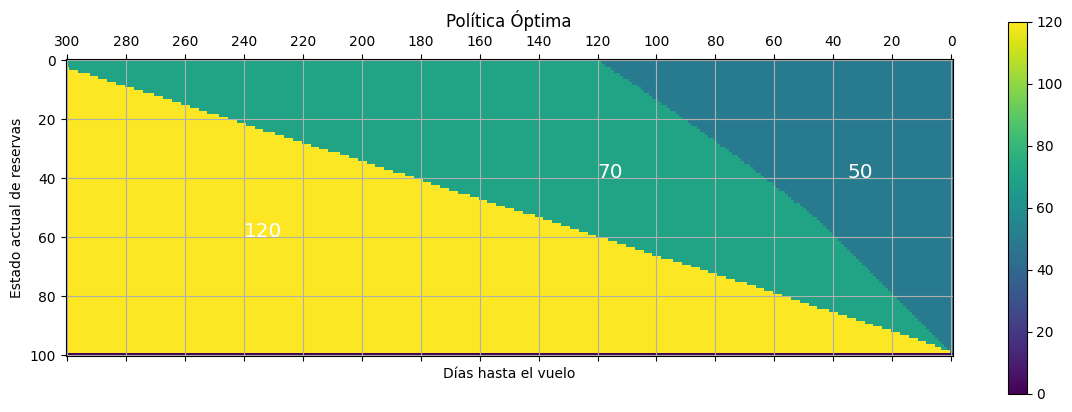
\includegraphics[trim={0mm 0mm 40mm 0mm}, clip,width=0.6\textwidth]{../Images/Figures/policymap.png}
\end{center}
\begin{itemize}
    \item \textbf{Umbrales en Precio:} Regiones de decisi\'on separadas por fronteras en el plano $(s, t)$.
    \item En modelos simplificados de otras aplicaciones, eso tambi\'en suele suceder:
\begin{itemize}
    \item \textbf{Gesti\'on de Inventarios:} Decisiones de reabastecimiento basadas en umbrales cr\'iticos.
    \item \textbf{Navegación:} Encontrar el camino m\'as corto (equivalente a minimizar costos acumulados).
\end{itemize}
\end{itemize}

\end{frame}

\begin{frame}{De la Política Óptima a Reglas de Negocio}

En muchos problemas reales, la política óptima es demasiado compleja para implementarse directamente.

\vspace{0.3cm}

La programación dinámica puede utilizarse para:

\begin{itemize}
\item descubrir la estructura de buenas decisiones;
\item identificar variables relevantes;
\item validar o mejorar heurísticas existentes;
\item diseñar reglas simples con desempeño cercano al óptimo.
\end{itemize}

\vspace{0.3cm}

\begin{block}{Ejemplo}
\begin{block}{Ejemplo}
En revenue management, los MDPs ayudaron a entender y perfeccionar heurísticas existentes, además de inspirar nuevas estrategias de protección de asientos y segmentación de tarifas que transformaron la industria.
\end{block}
\end{block}

\end{frame}


% --- SLIDE: PROGRAMACIÓN DINÁMICA ---
\begin{frame}{Resumiendo Hasta Ahora}
\begin{itemize}
\item Calculamos la funci\'on valor $V^*$ recursivamente:
\visible<2->{
\begin{block}{Algoritmo con Horizonte $T$}
\begin{enumerate}
\item<3-> \textbf{Base:} Para $t = T$, calculamos la recompensa final: $V_T^*(x) = \max_a r_a(x).$
\item<4-> \textbf{Inducci\'on:} Para $t = T-1, \dots, 0$, resolvemos:
\[ V^*_t(x) =  \max_{a \in A} \left\{ r_a(x) +\sum_y P_a(x,y) V_{t+1}^*(y) \right\} \]
\end{enumerate}
\end{block}}
\item<6-> La pol\'itica \'optima $u^*_t(x)$ es el argumento que maximiza dicha expresión.
\end{itemize}
\end{frame}

% --- SLIDE: EJEMPLO PESCA ---
\begin{frame}{Ejemplo: Pesca de Salmones}
Cada a\~no debemos decidir cu\'anto salm\'on pescar en una determinada \'area. Cada ejemplar genera una ganancia fija, pero una pesca excesiva impacta negativamente en la poblaci\'on del a\~no siguiente.

\vspace{0.3cm}
El objetivo es maximizar la ganancia total acumulada. \textquestiondown C\'omo modelamos este problema?

\vspace{0.4cm}
\visible<2->{Consideremos una versi\'on simplificada para visualizar el proceso:
\begin{itemize}
    \item<3-> \textbf{Acciones:} En cada a\~no, decidimos si pescar o no una proporci\'on fija de la biomasa.
    \item<4-> \textbf{Estados:} La poblaci\'on se categoriza en 4 niveles: \textit{Vac\'io, Bajo, Mediano} y \textit{Alto}.
\end{itemize}}
\end{frame}

% --- SLIDE: MODELO ---
\begin{frame}{Pesca de Salmones: Modelo}
\begin{center}
\mode<beamer>{
\only<1>{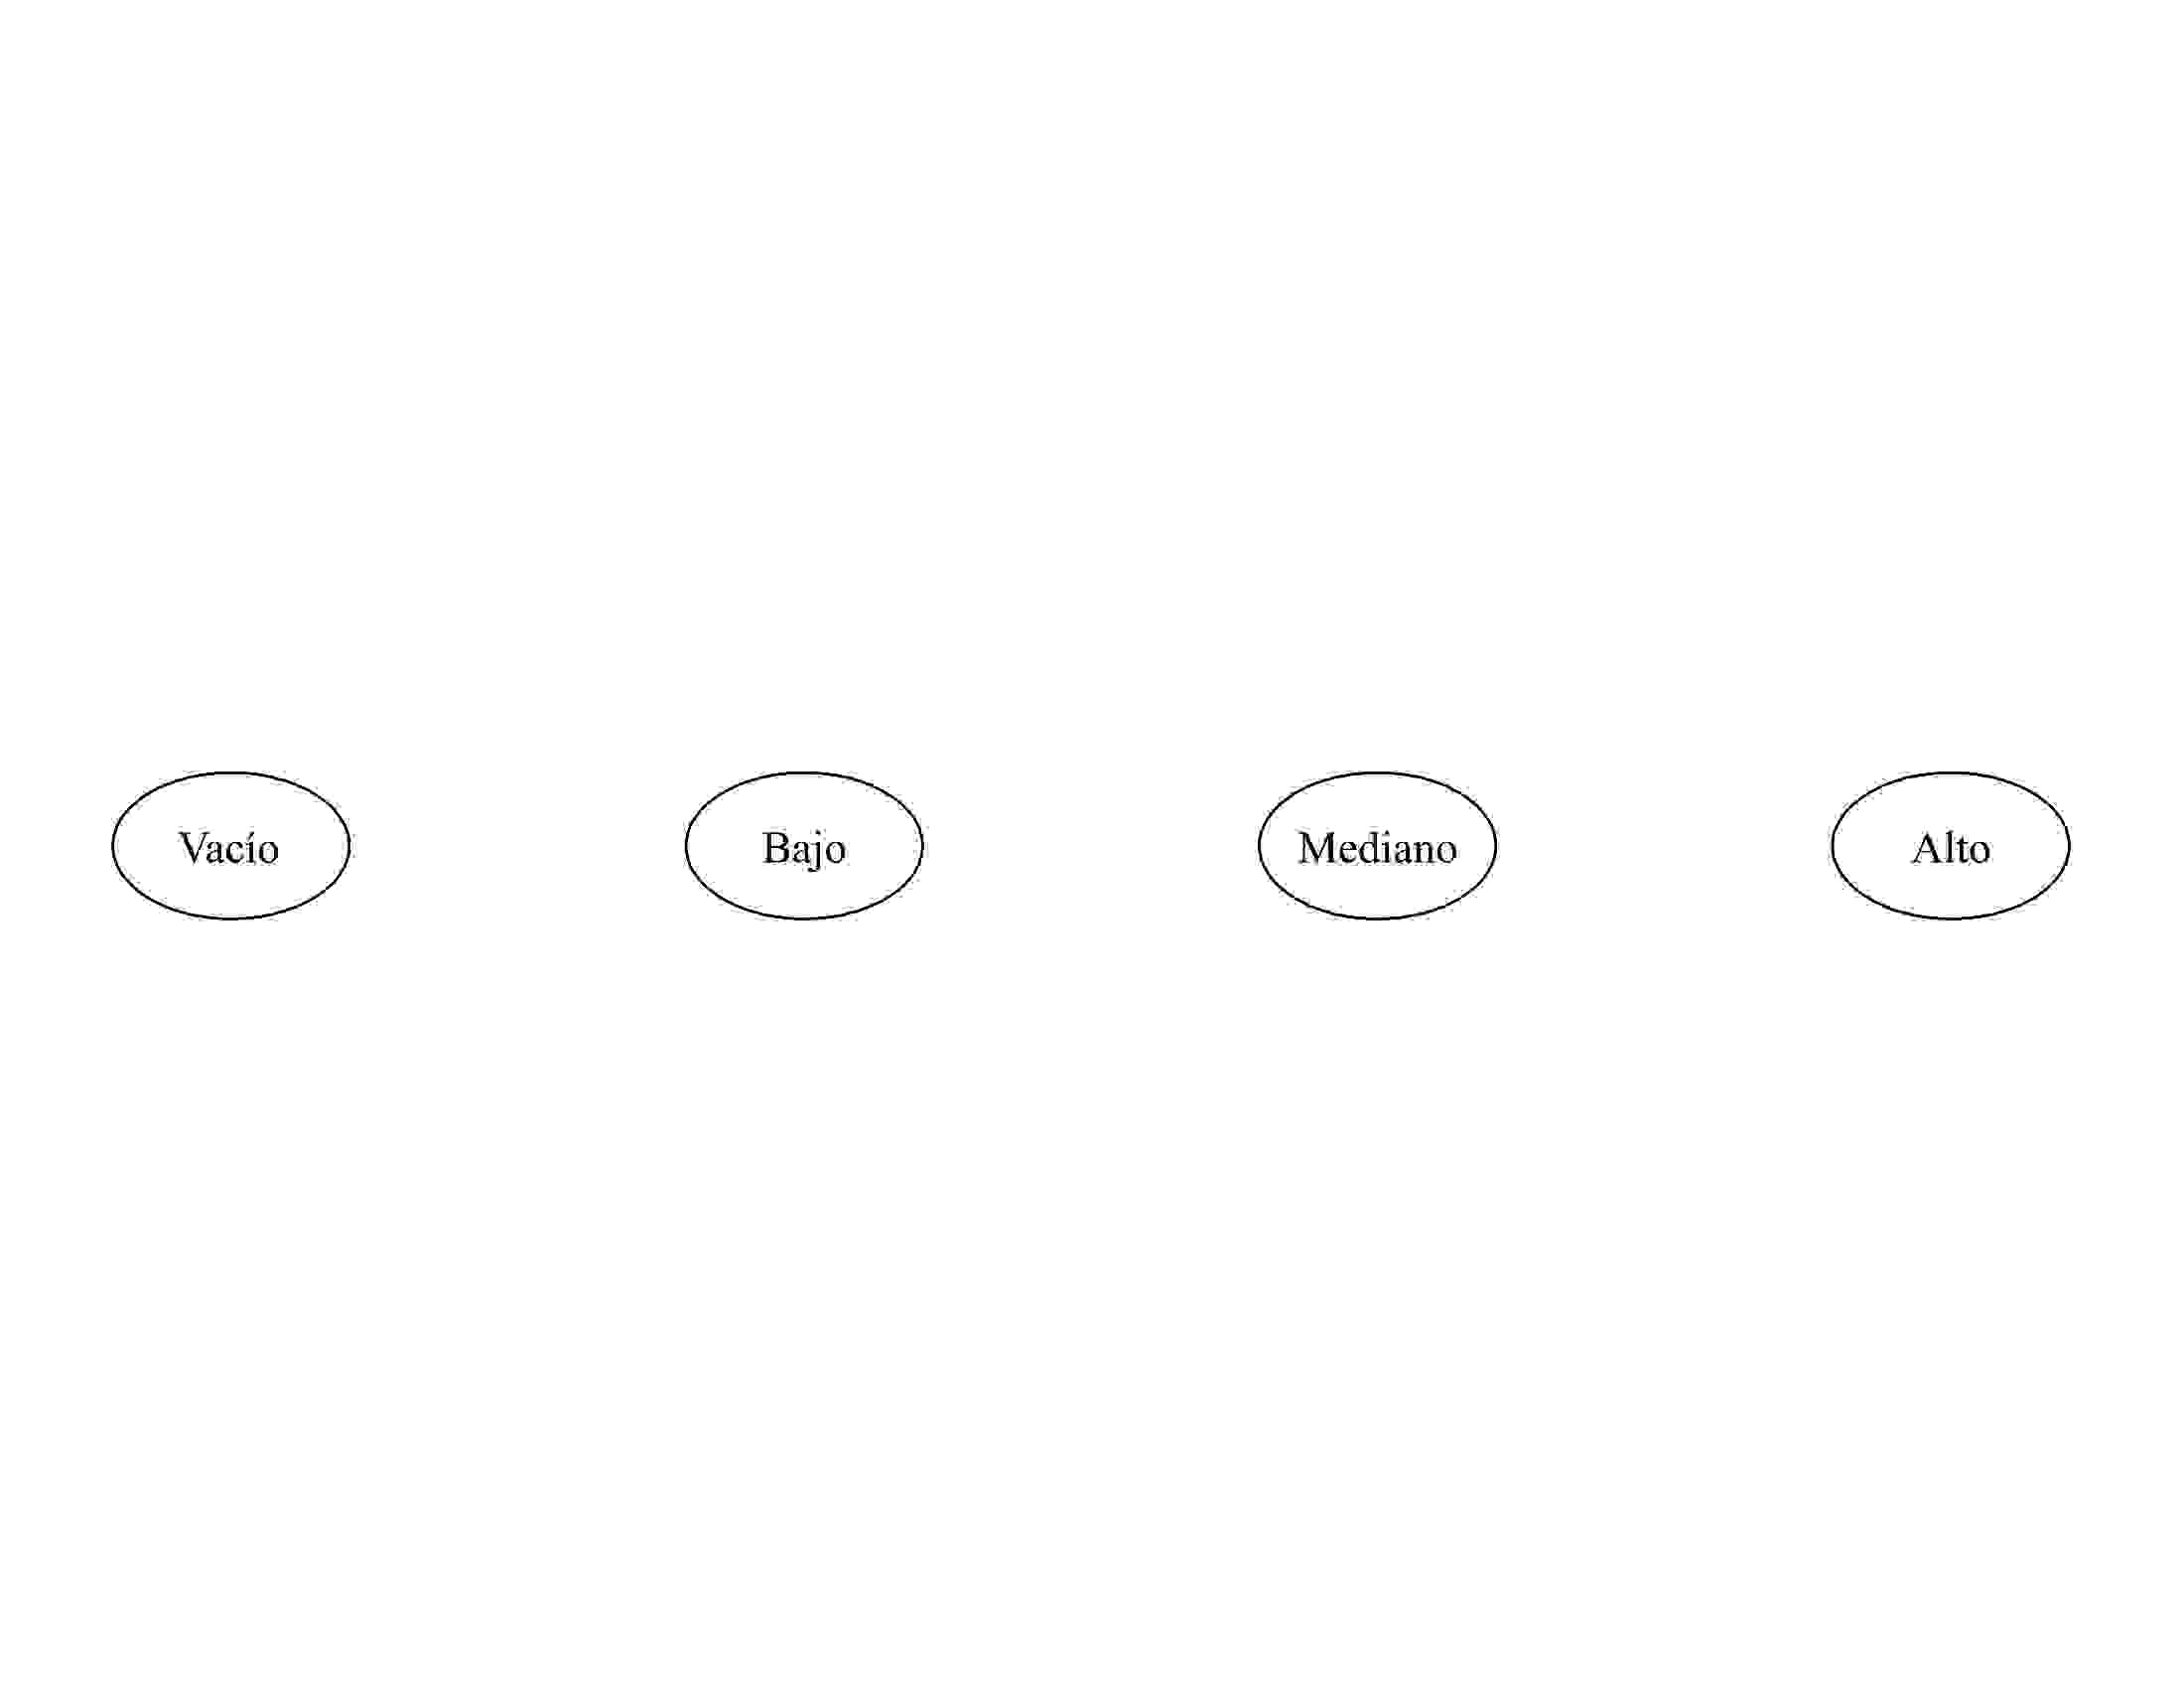
\includegraphics[width=1\textwidth]{../Images/SalmonFishing/SalmonFishing1.jpg}}
\only<2>{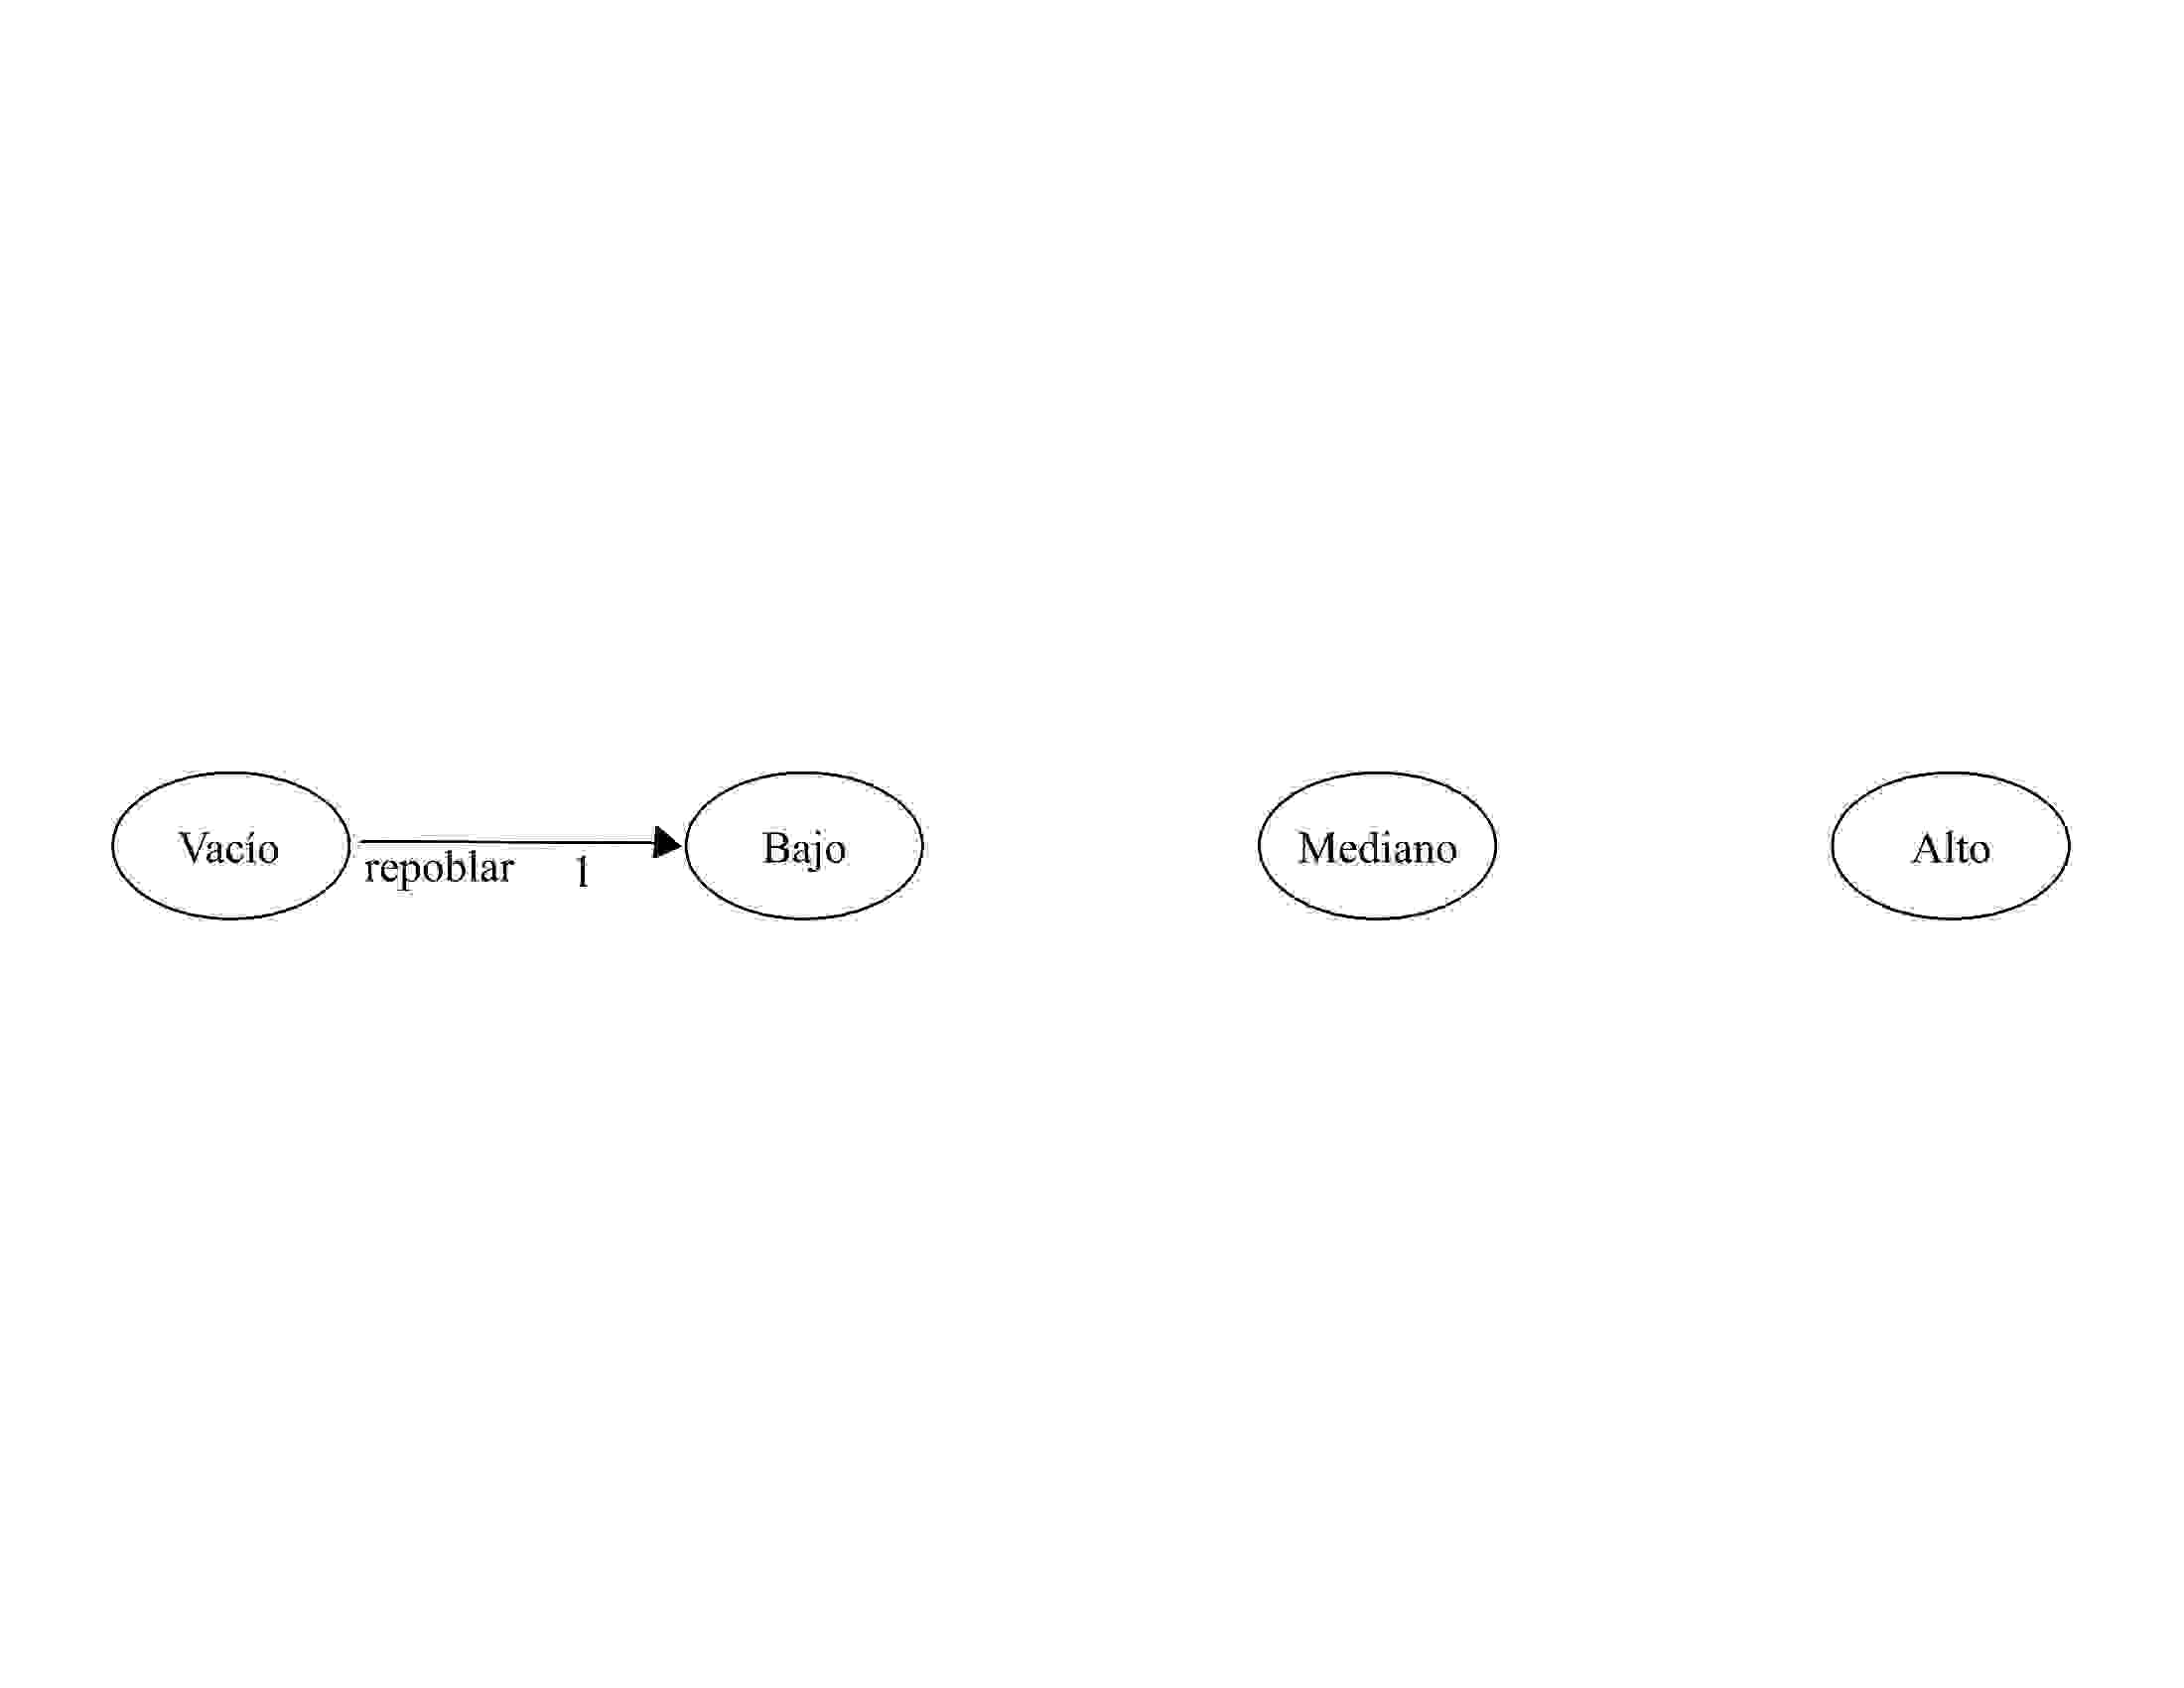
\includegraphics[width=1\textwidth]{../Images/SalmonFishing/SalmonFishing2.jpg}}
\only<3>{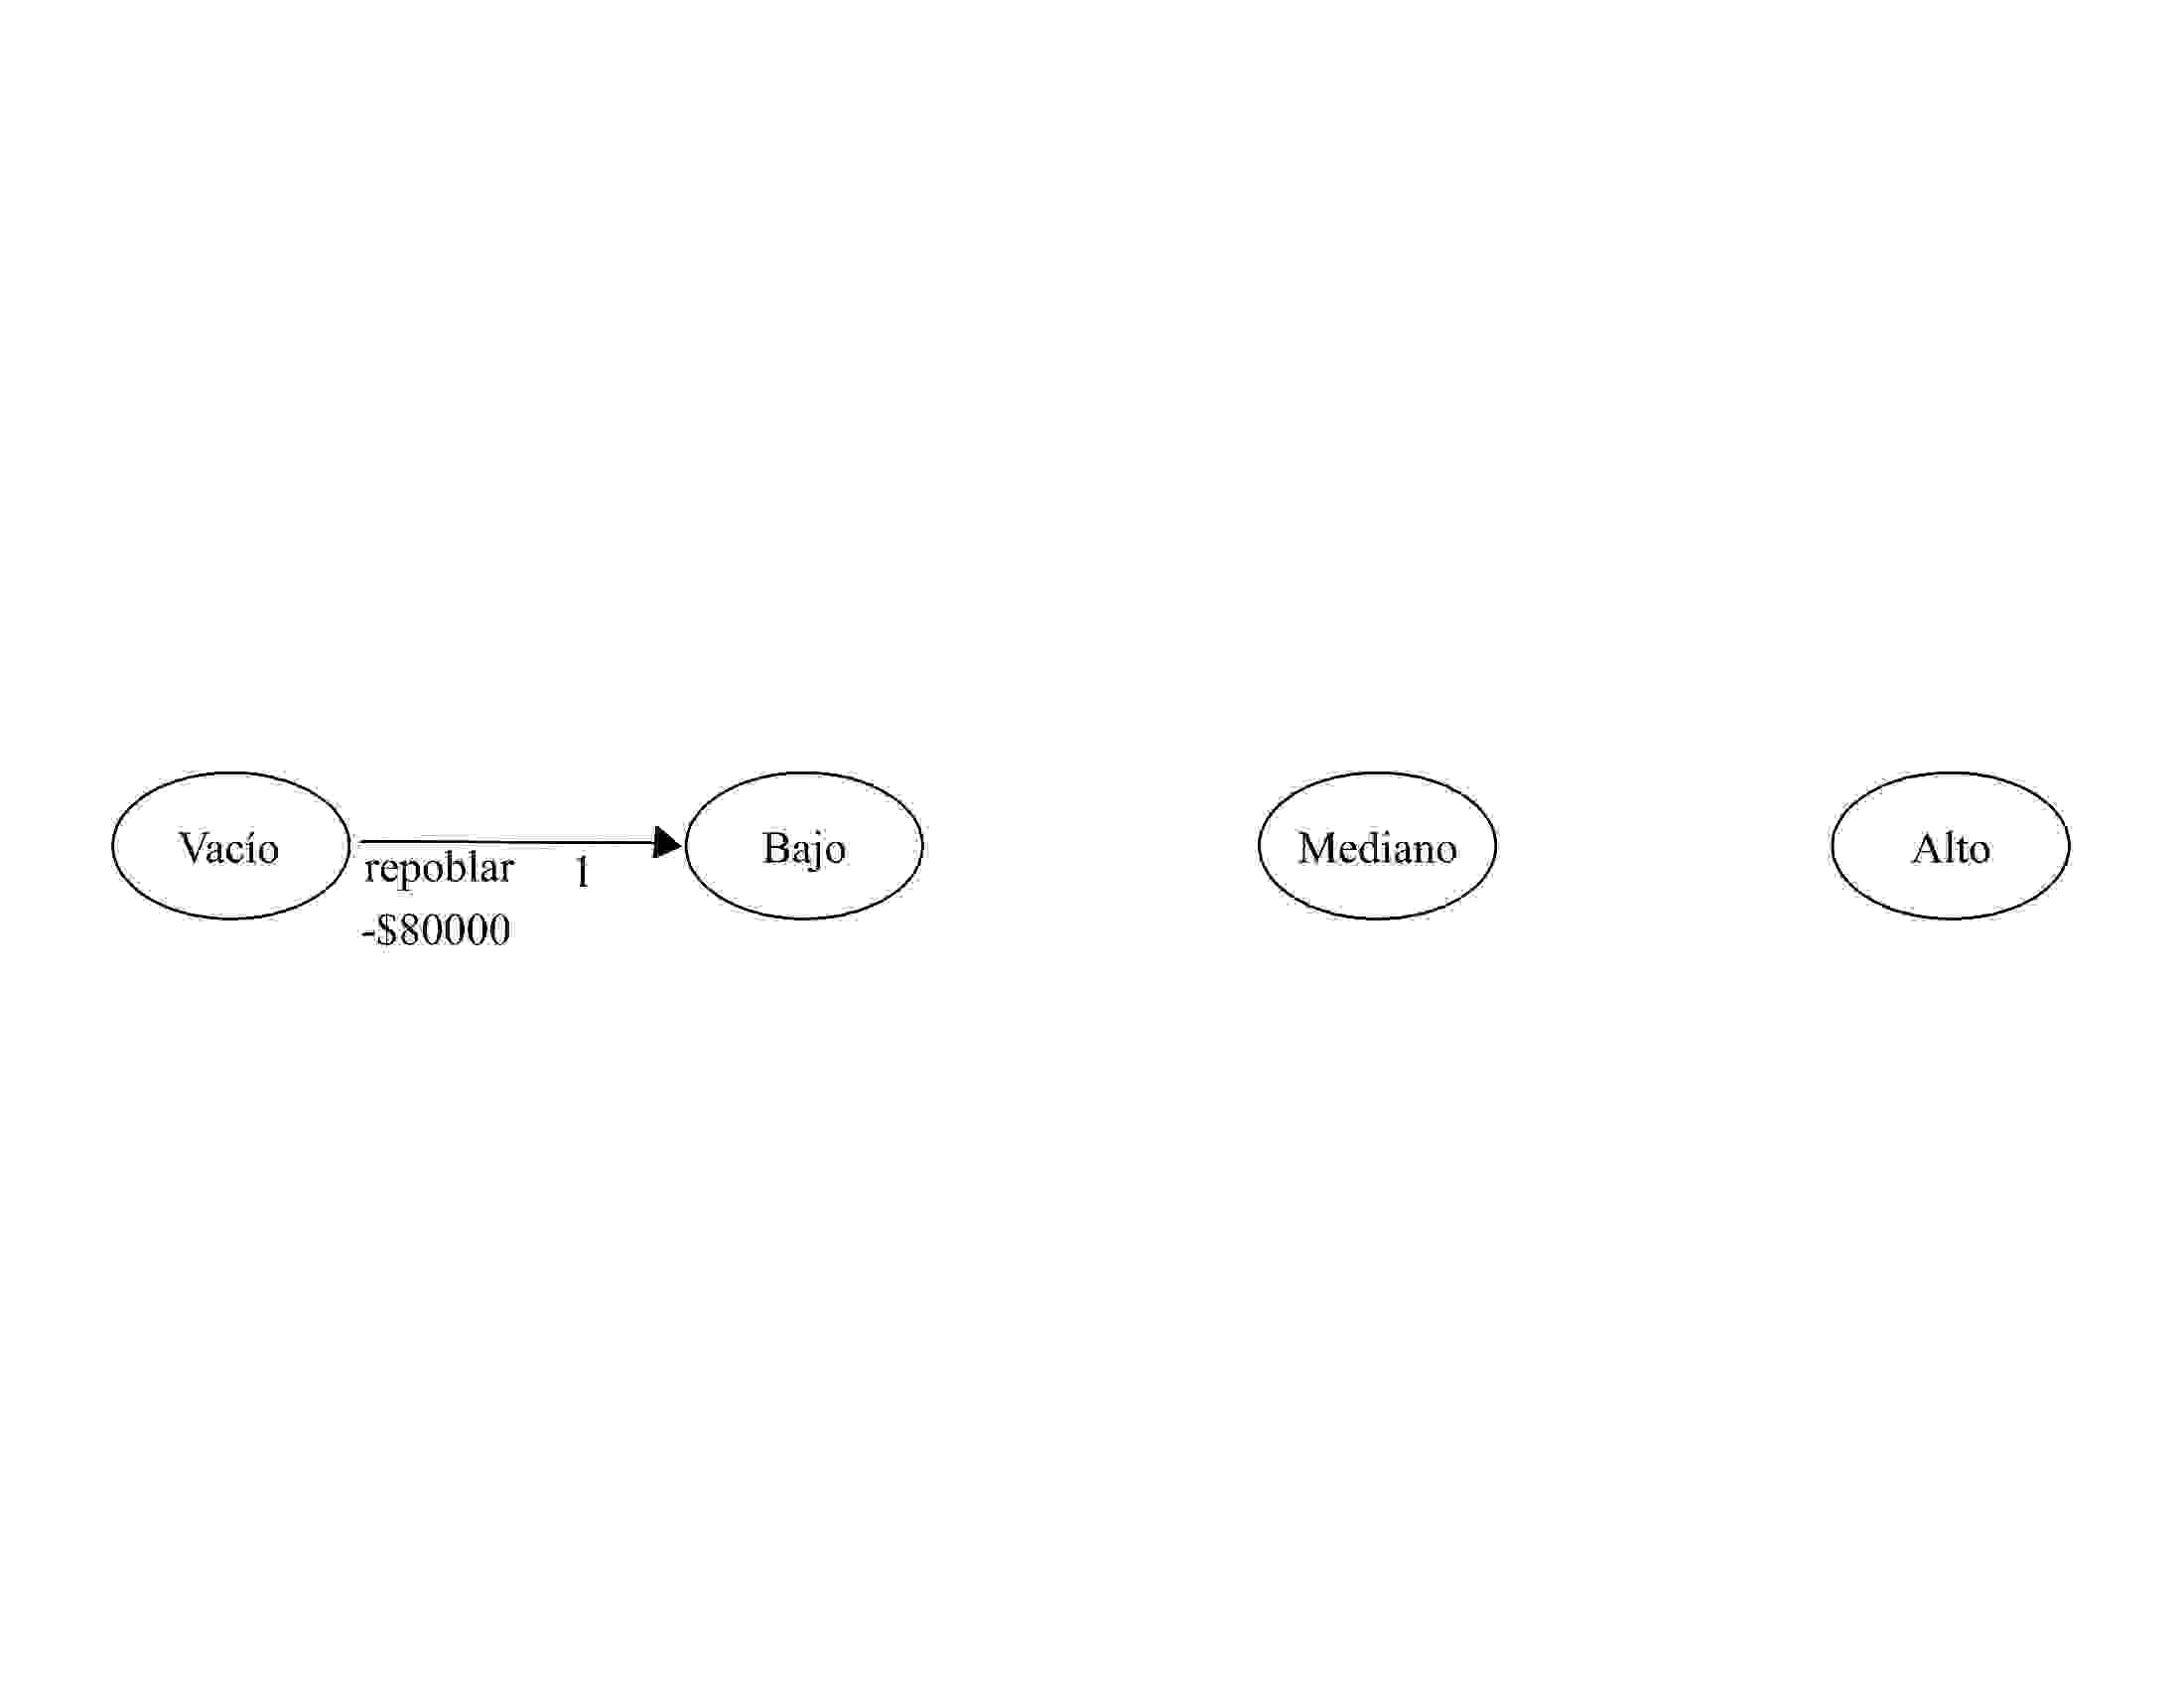
\includegraphics[width=1\textwidth]{../Images/SalmonFishing/SalmonFishing3.jpg}}
\only<4>{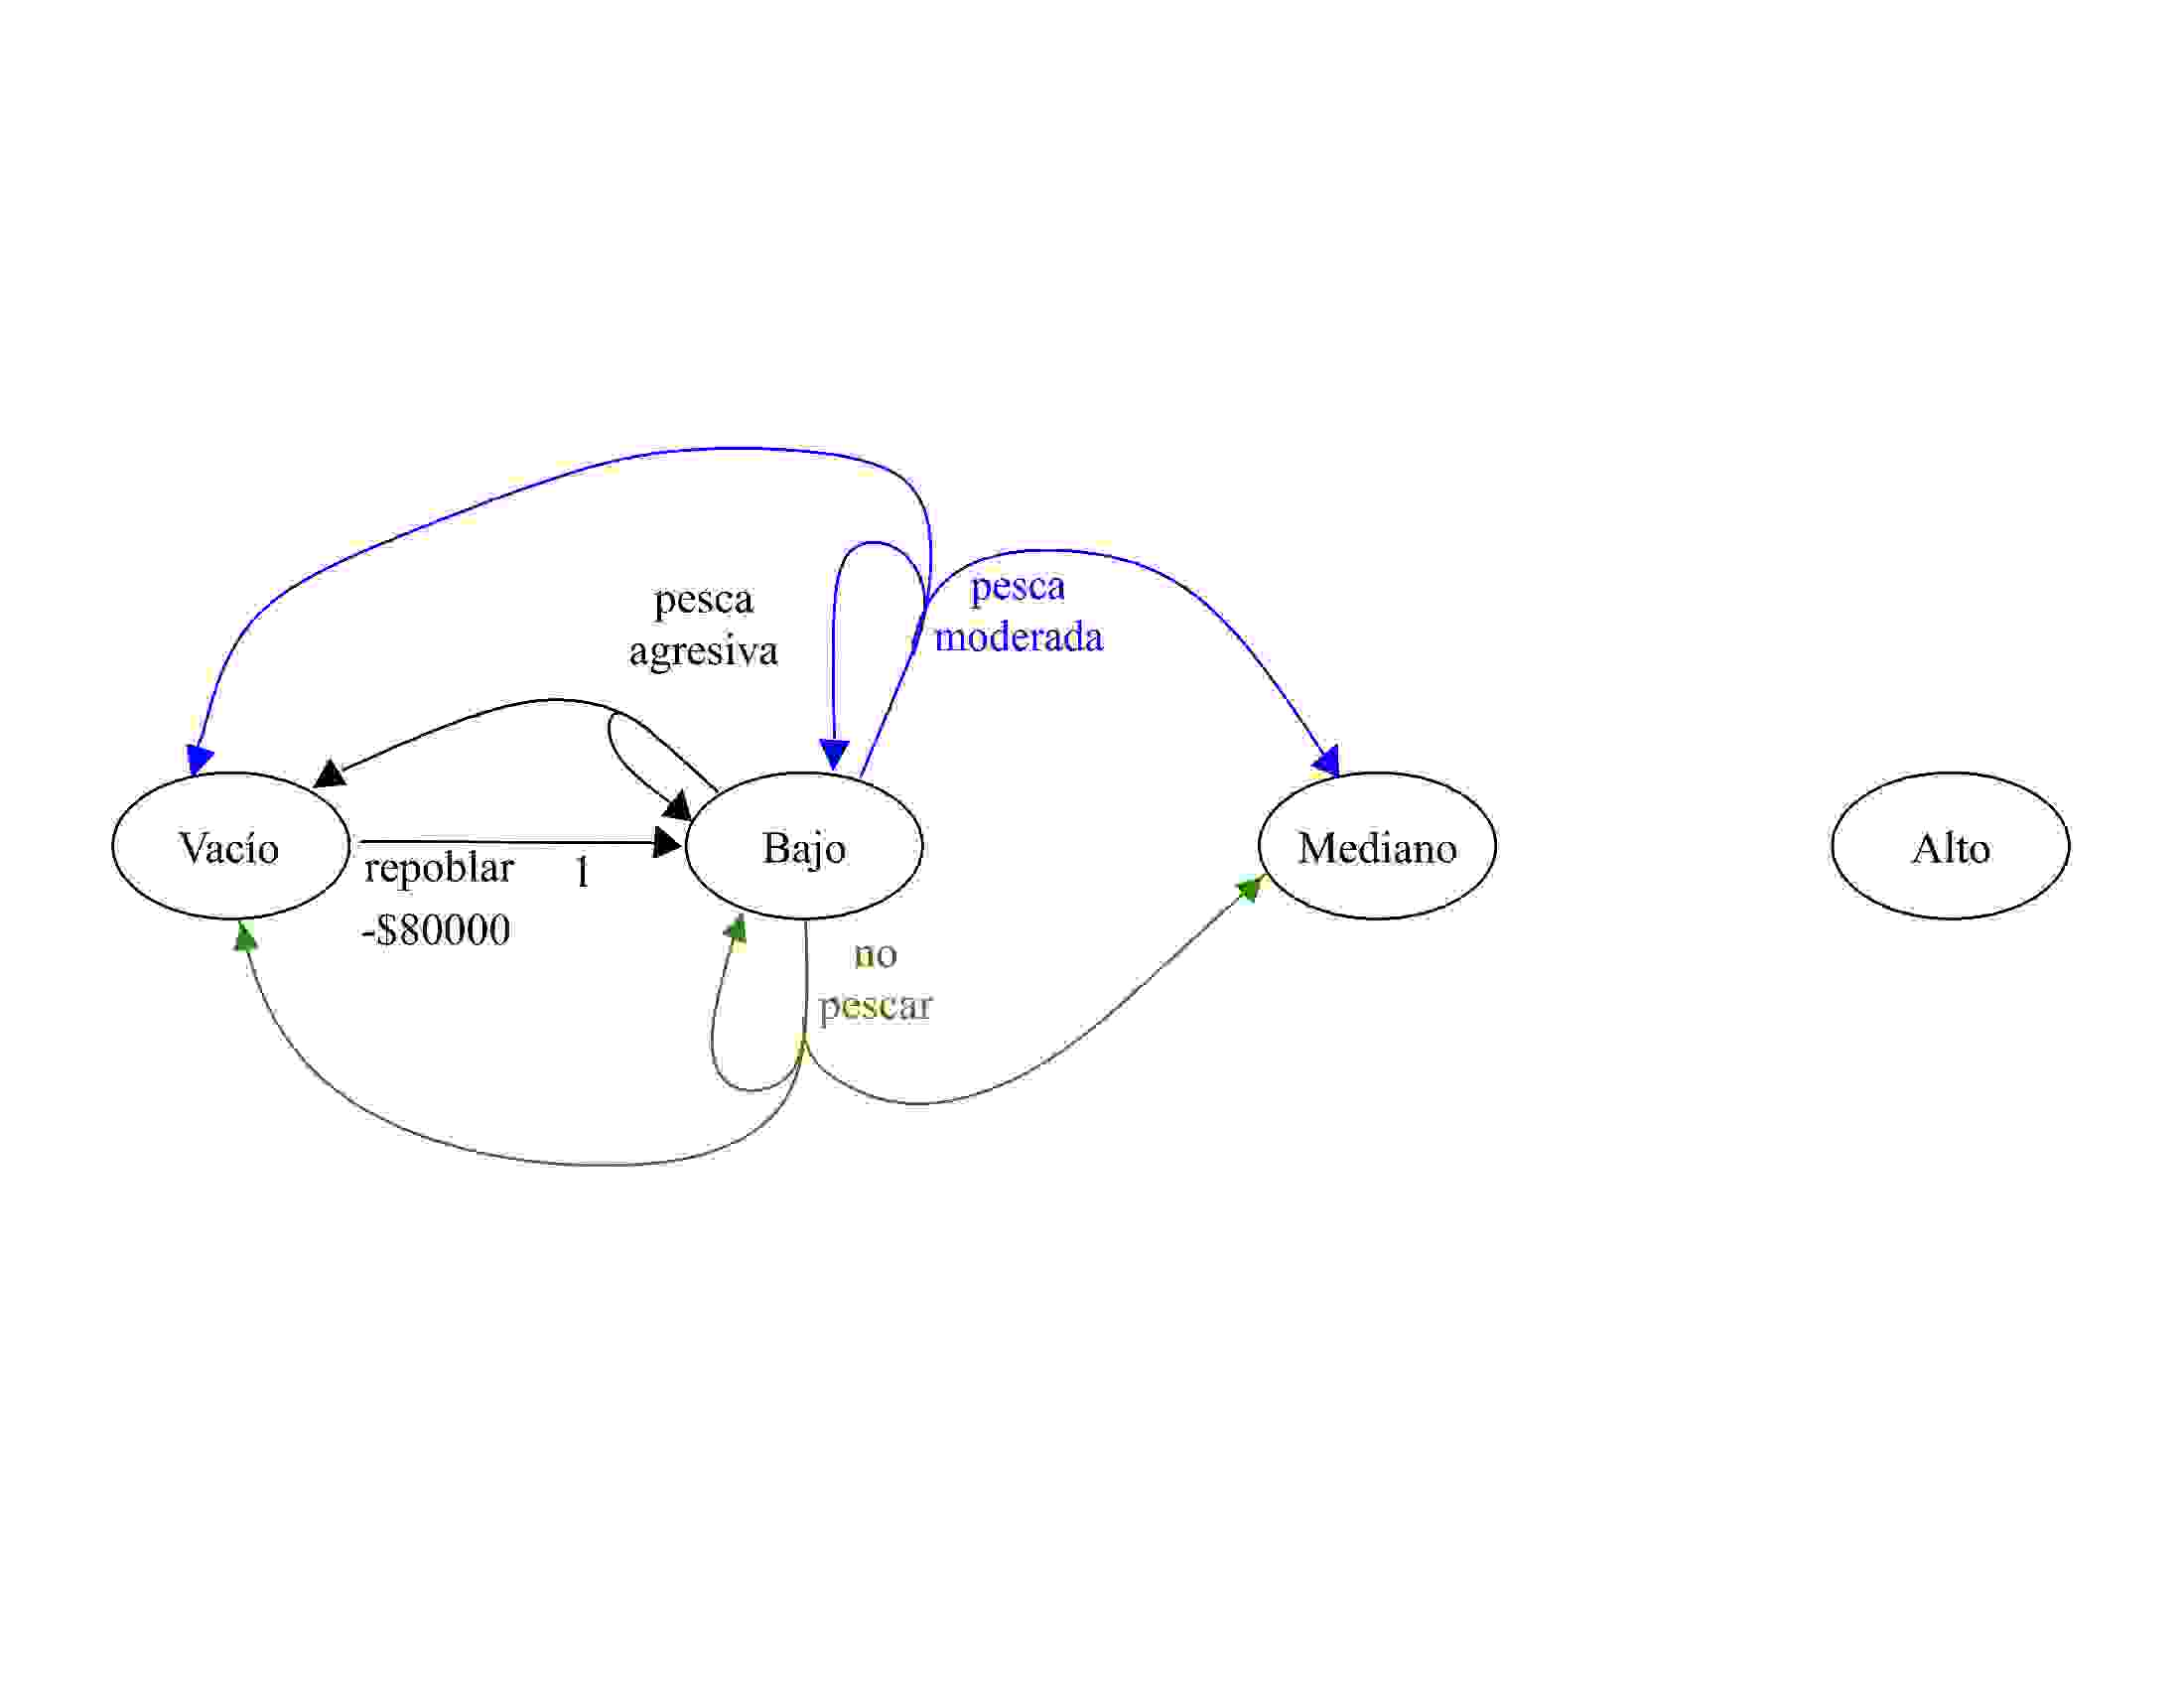
\includegraphics[width=1\textwidth]{../Images/SalmonFishing/SalmonFishing4.jpg}}
\only<5>{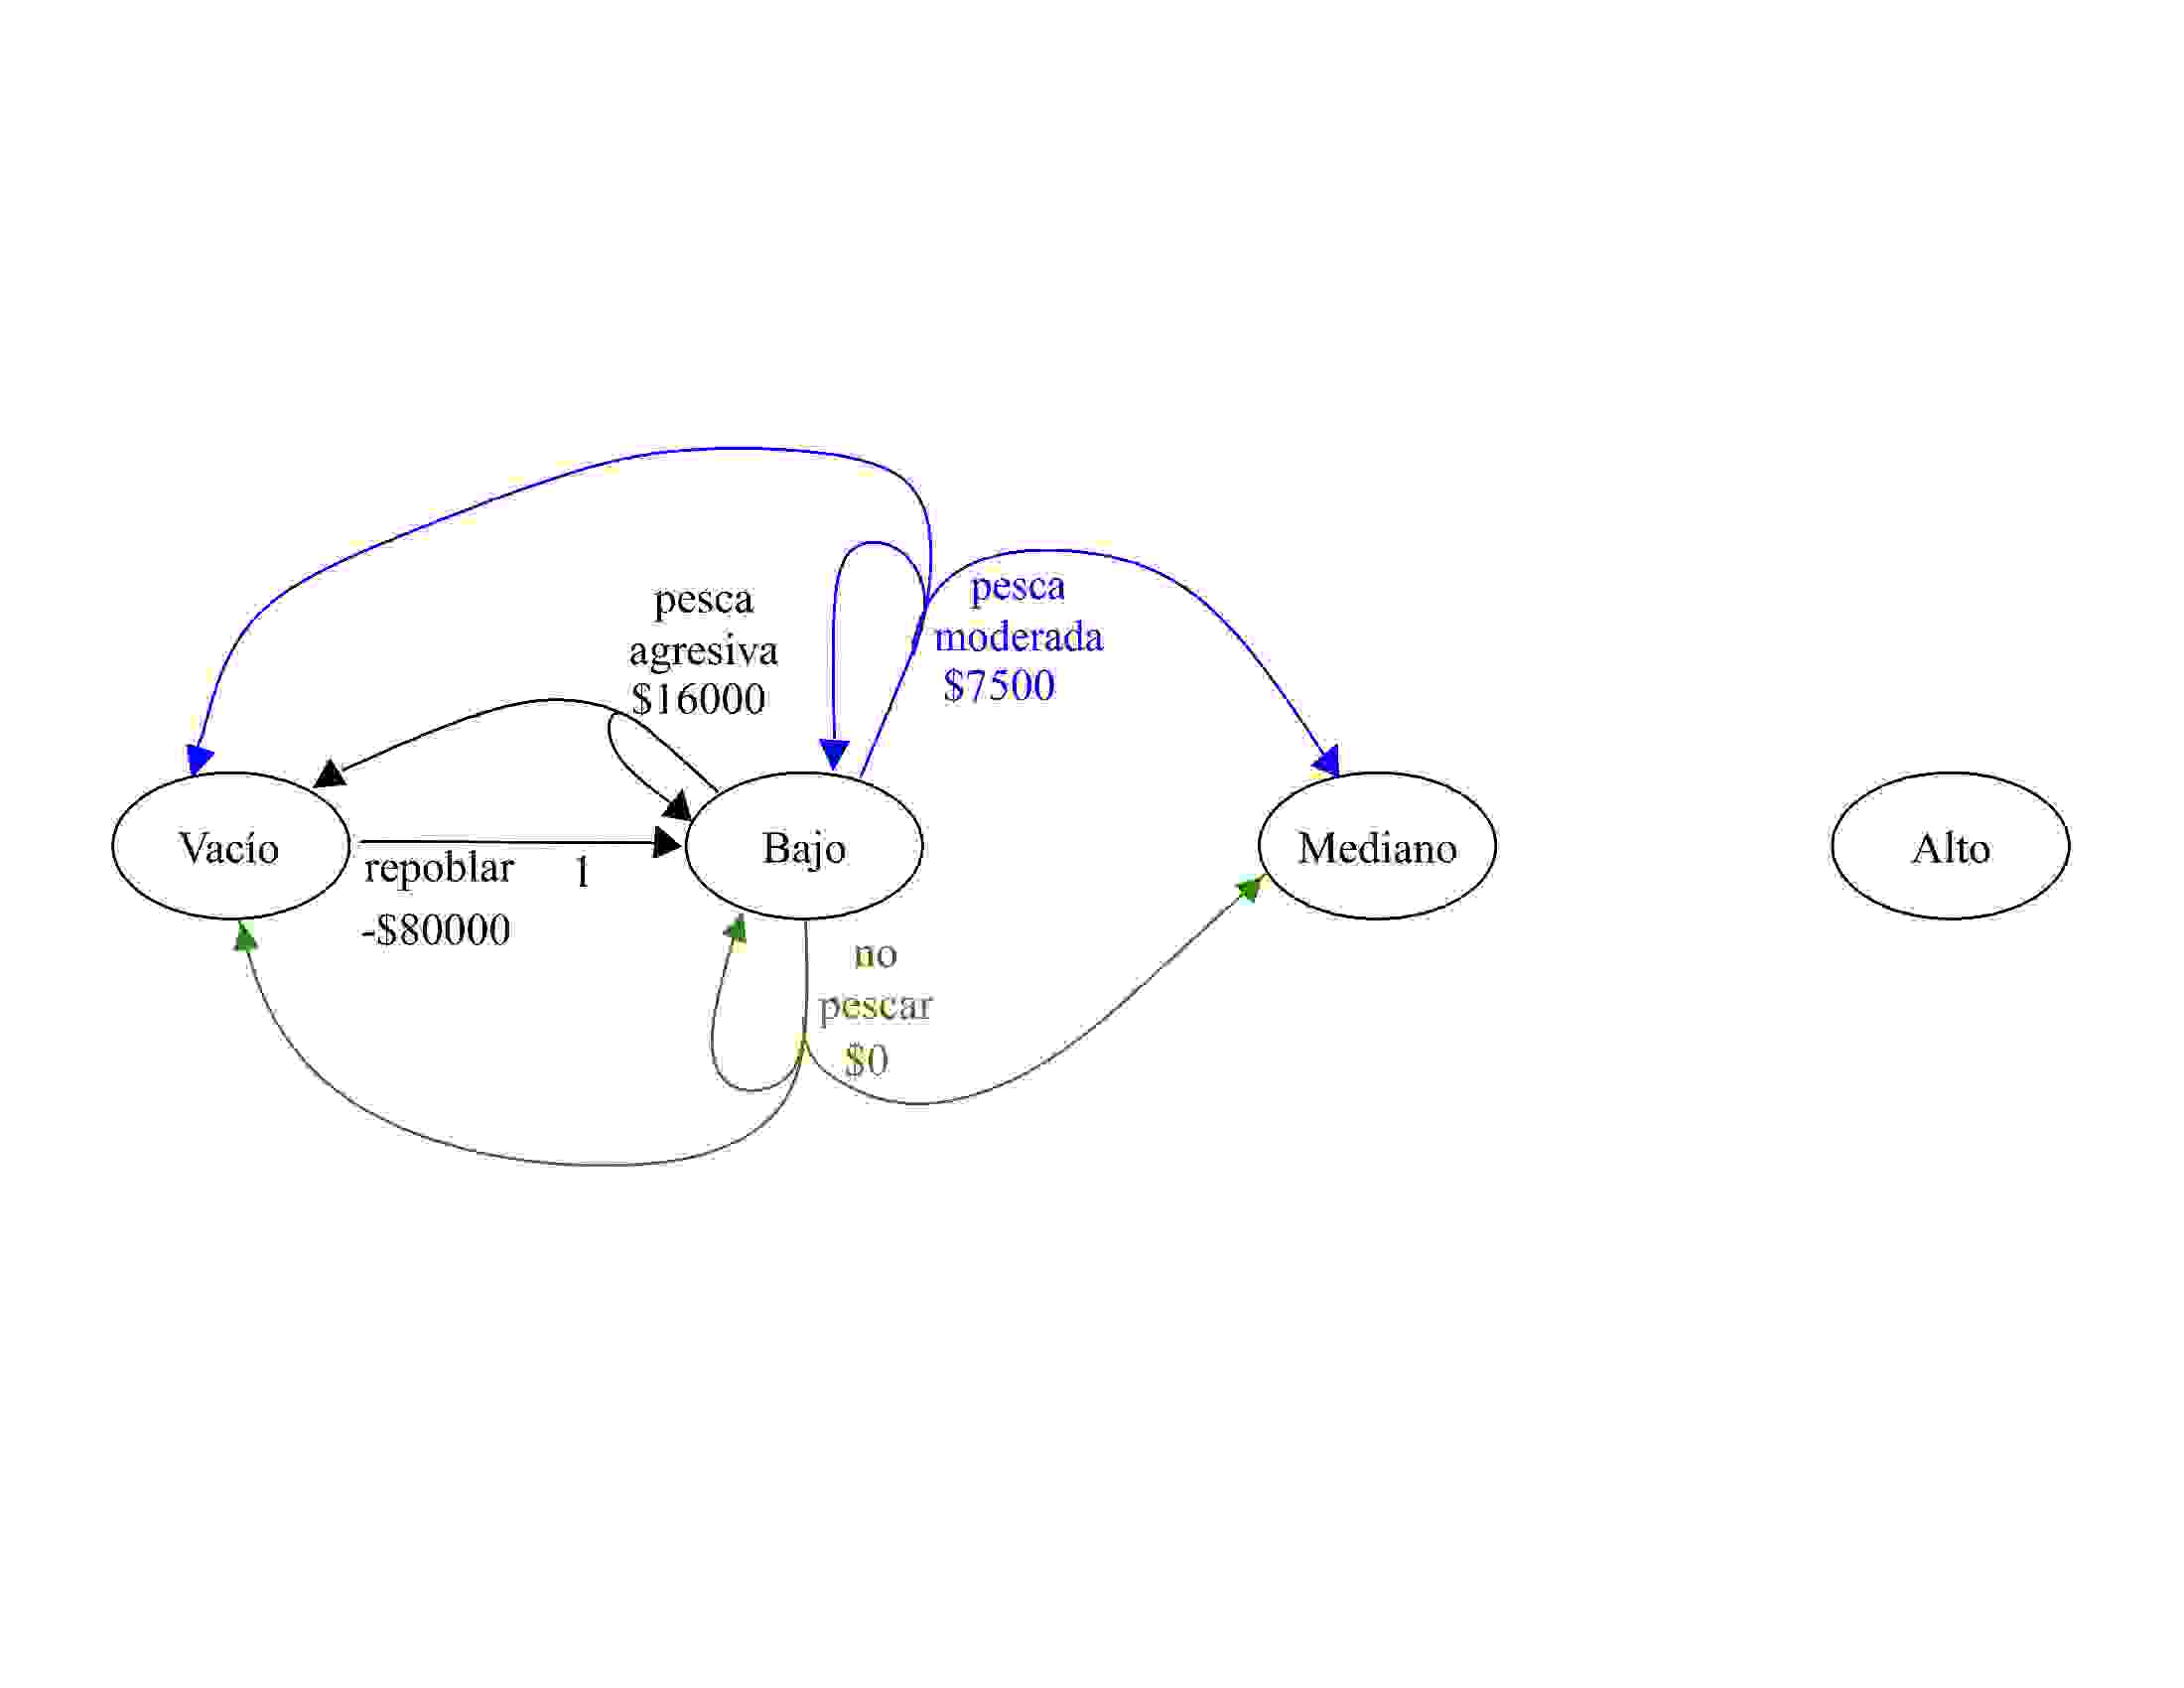
\includegraphics[width=1\textwidth]{../Images/SalmonFishing/SalmonFishing5.jpg}}
\only<6>{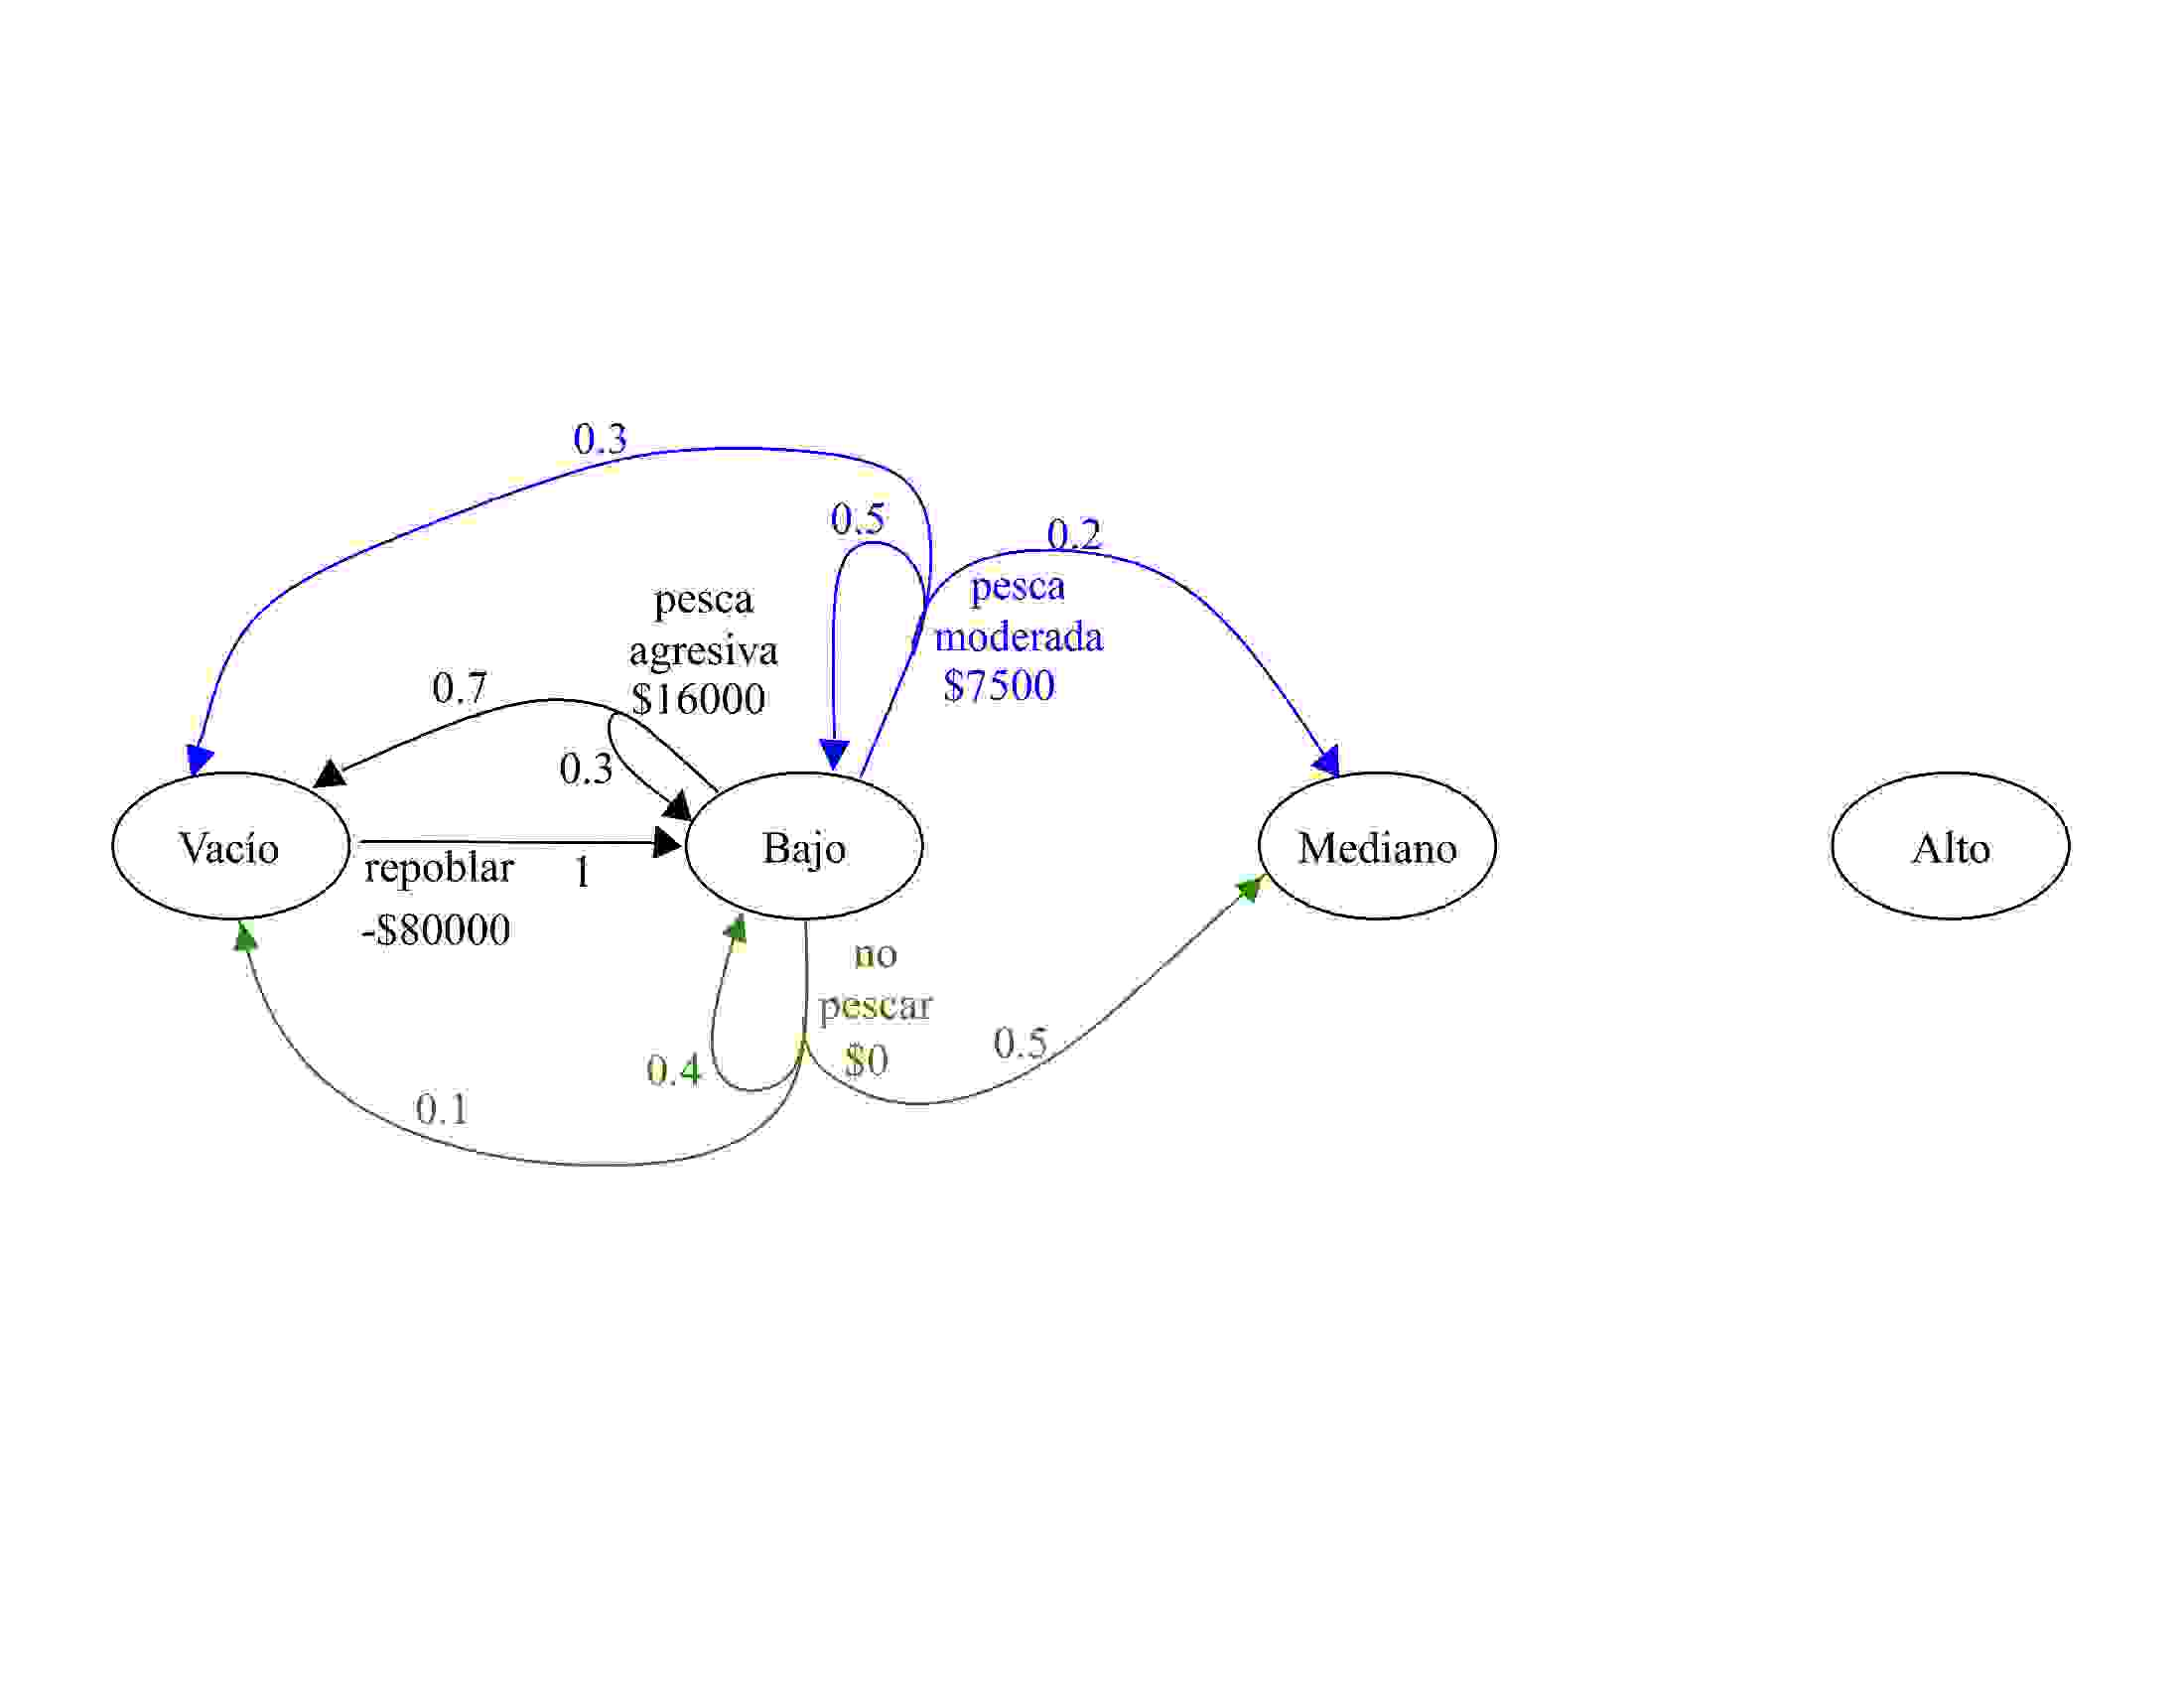
\includegraphics[width=1\textwidth]{../Images/SalmonFishing/SalmonFishing6.jpg}}}
\only<7->{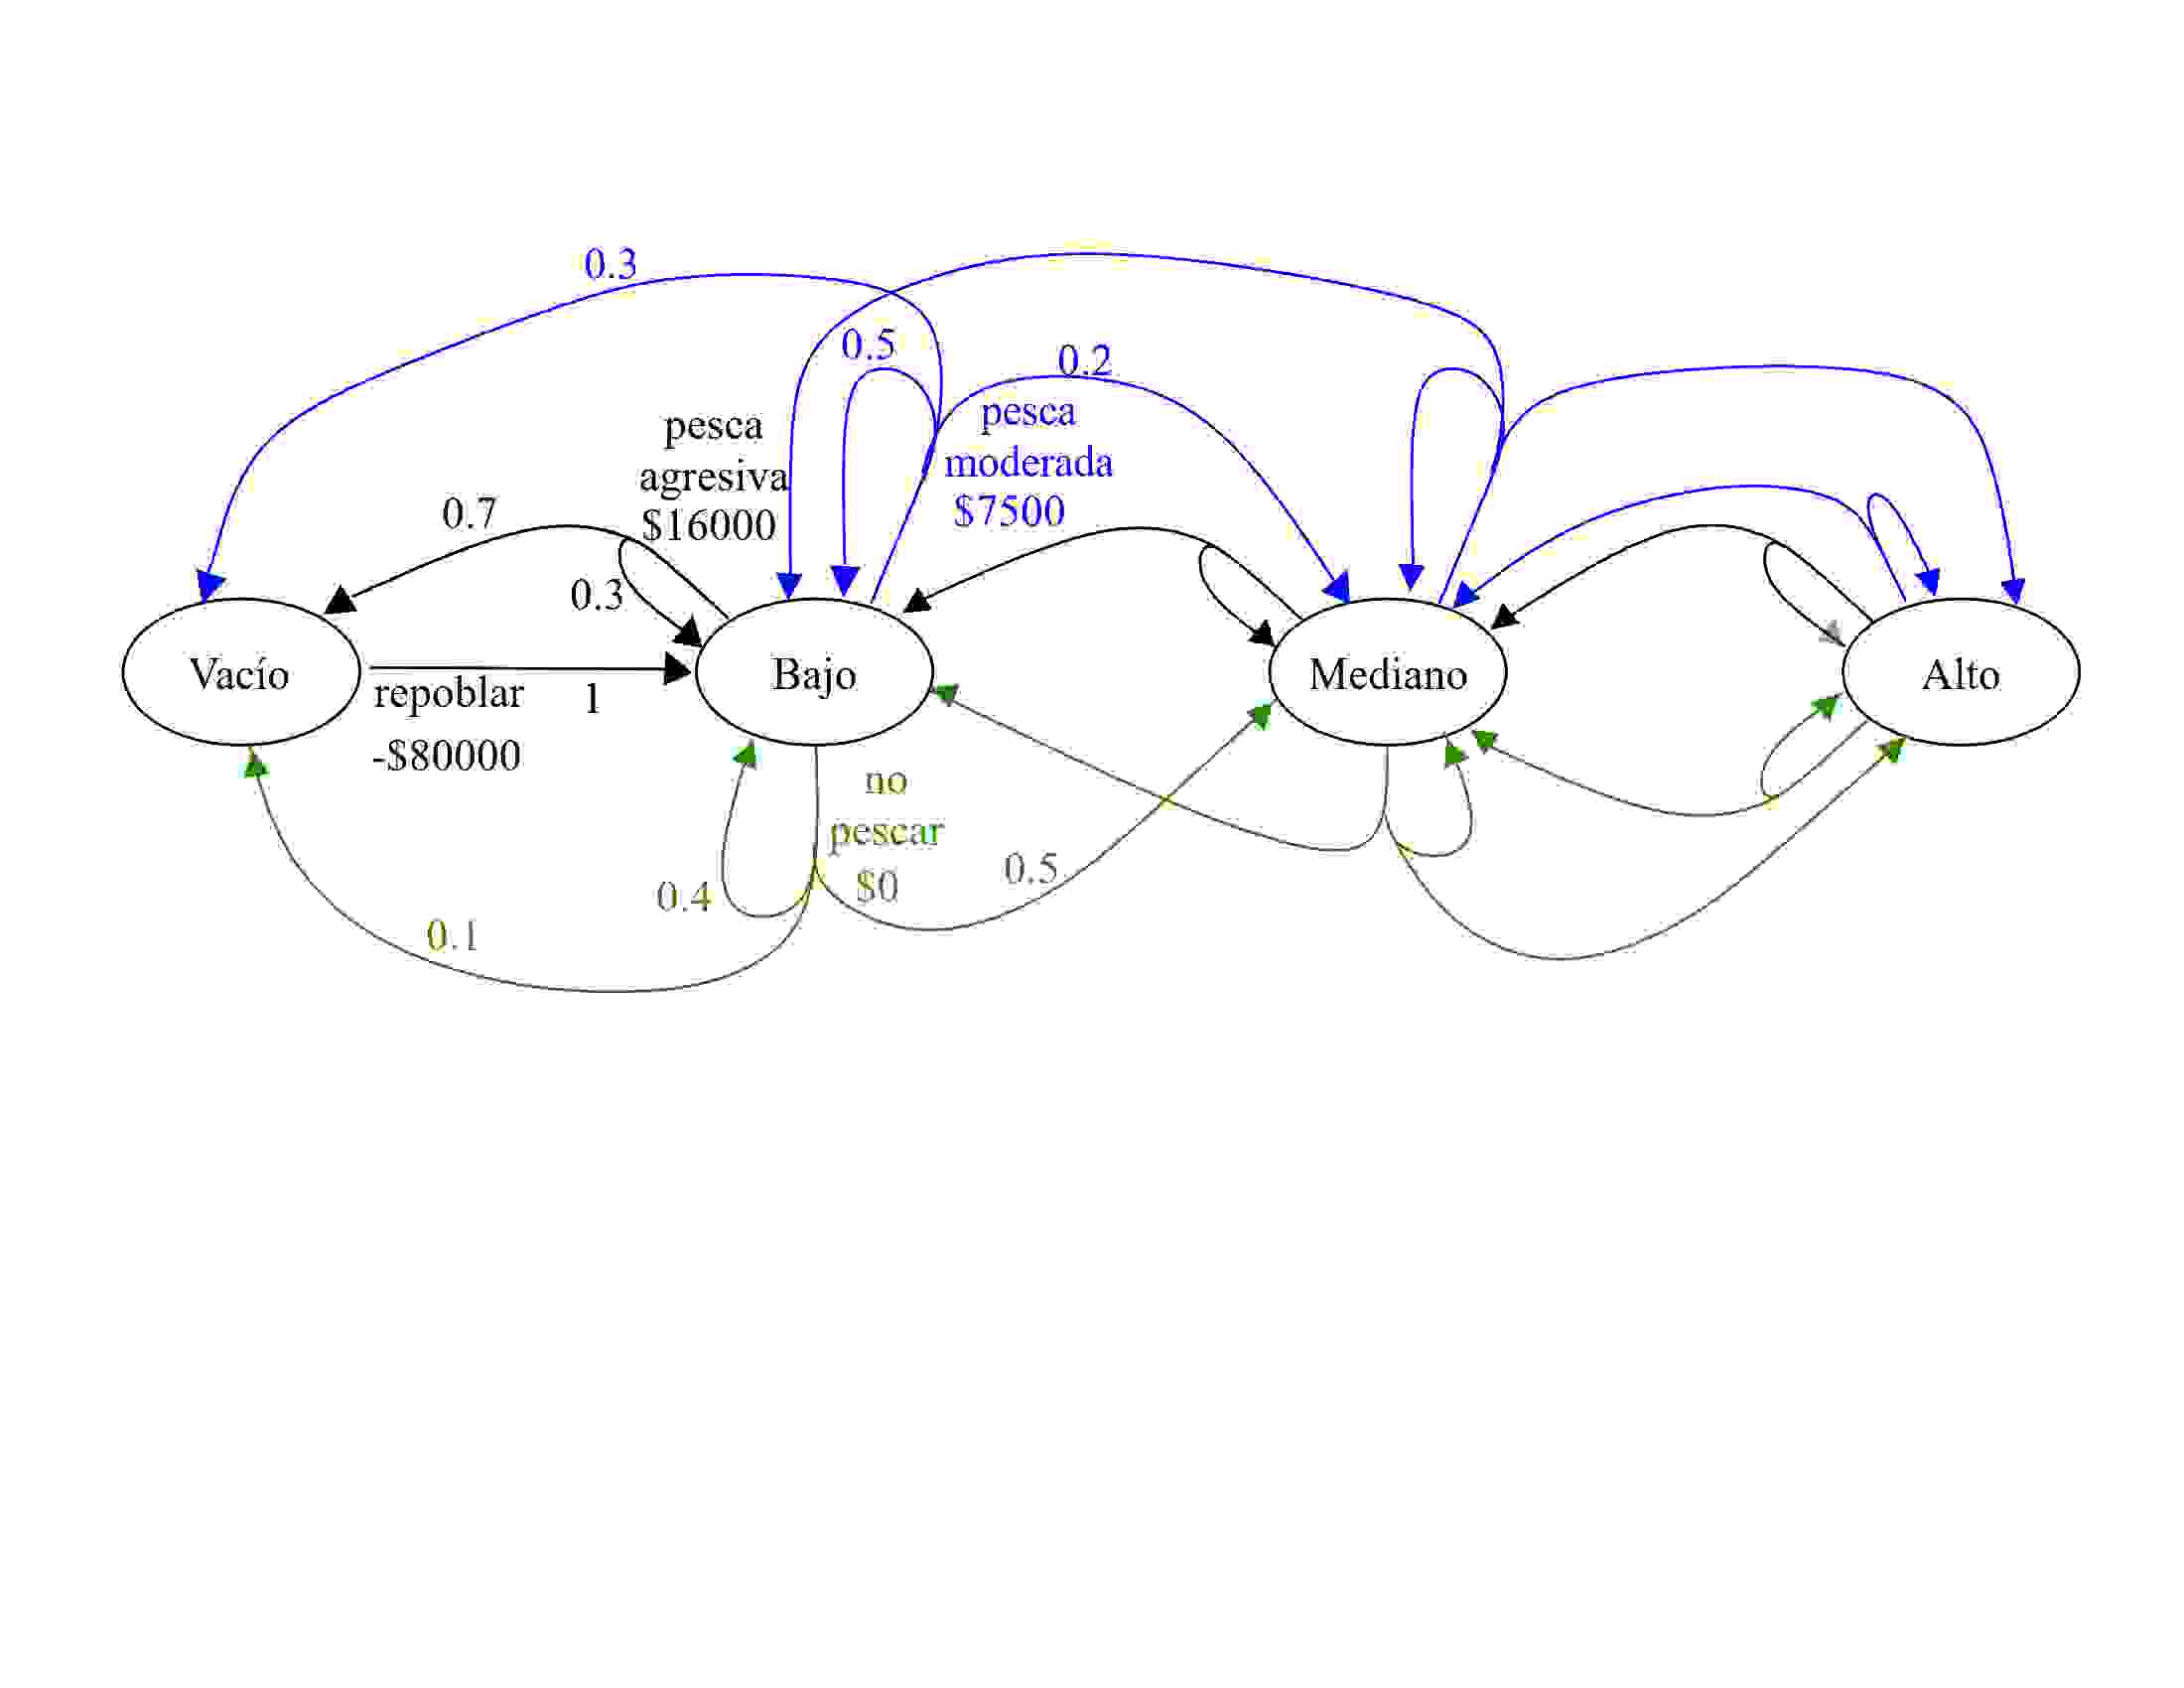
\includegraphics[width=1\textwidth]{../Images/SalmonFishing/SalmonFishing7.jpg}}
\end{center}
\vspace{-3cm}
\only<8>{\centering \textbf{\textquestiondown Qu\'e decisiones tomar?} Vamos a resolver el problema con Python.}
\end{frame}

% --- SLIDE: RESULTADOS ---
\begin{frame}{Pesca de Salmones: Resultados}
\begin{itemize}
    \item Visualizaci\'on de la pol\'itica \'optima:
    \begin{itemize}
        \item<2-> La acci\'on \'optima depende tanto del \textbf{estado} como del \textbf{tiempo restante}.
    \end{itemize}
    \item<3-> \textquestiondown C\'omo impacta la elecci\'on del horizonte $T$ en nuestras decisiones?
\end{itemize}
\begin{center}
    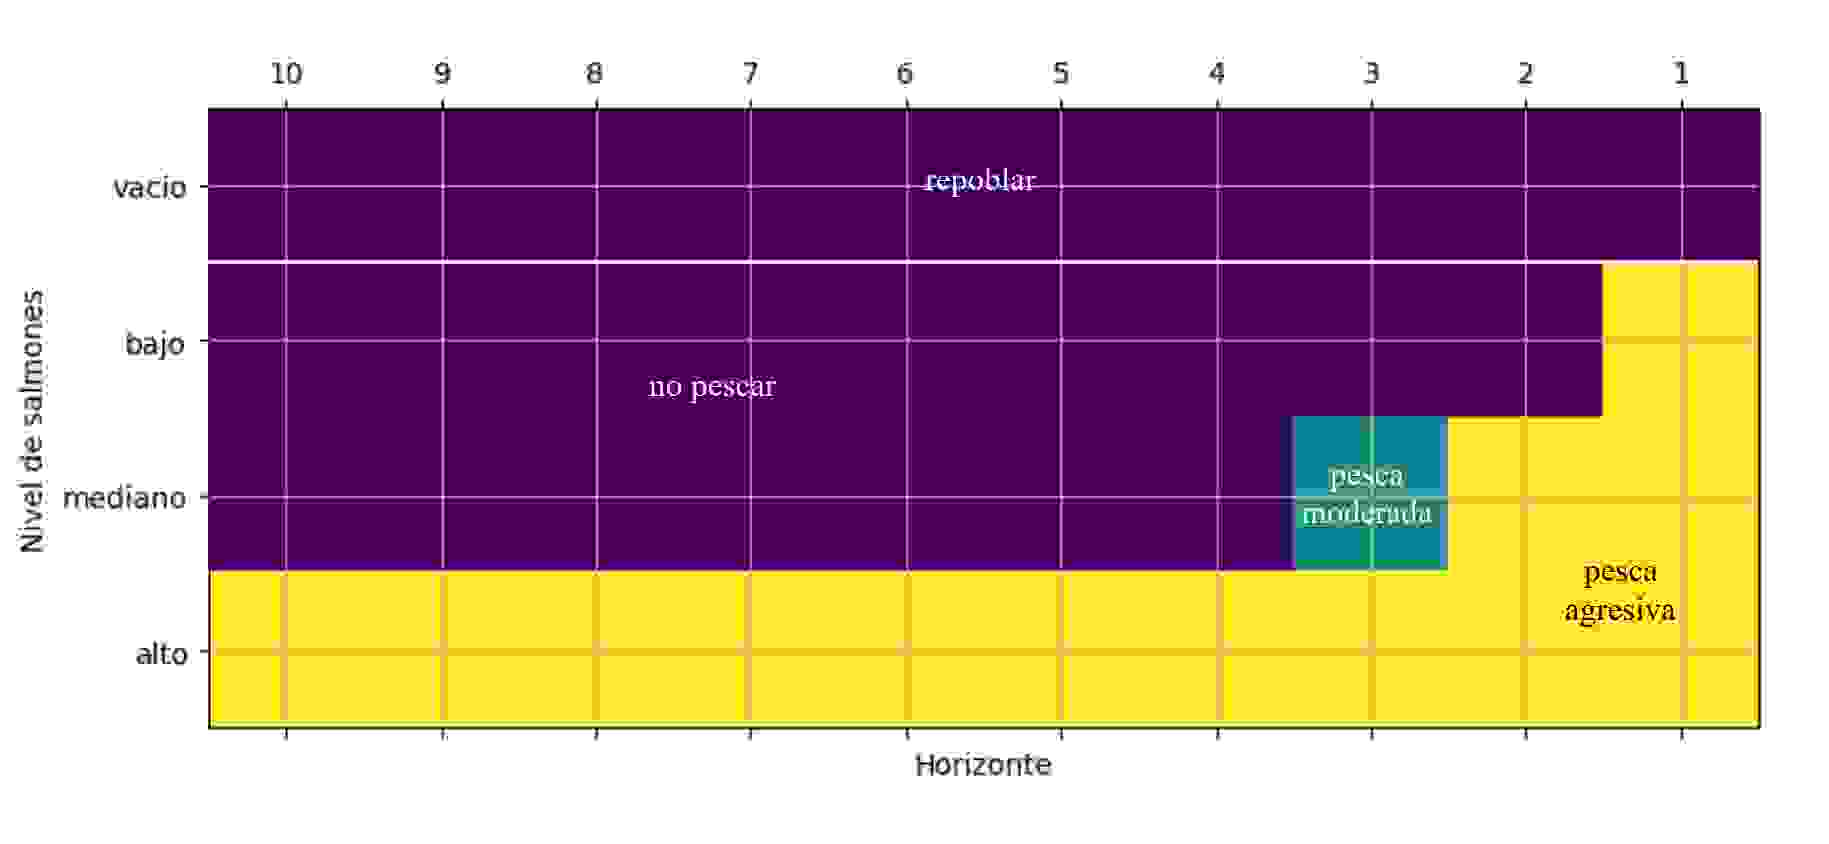
\includegraphics[width=1\textwidth]{../Images/SalmonFishing/SalmonFishingPolicy1.jpg}
\end{center}
\end{frame}

% --- SLIDE: OPCIÓN REPOBLAR ---
\begin{frame}{Pesca de Salmones: Opci\'on de No Repoblar}
\begin{itemize}
    \item<1-> Si en el estado \textit{vac\'io} existe la opci\'on de \textbf{no repoblar}, \textquestiondown c\'omo cambia el an\'alisis? \textquestiondown Bajo qu\'e condiciones es rentable repoblar?
\end{itemize}
\begin{center}
\mode<beamer>{
\only<1>{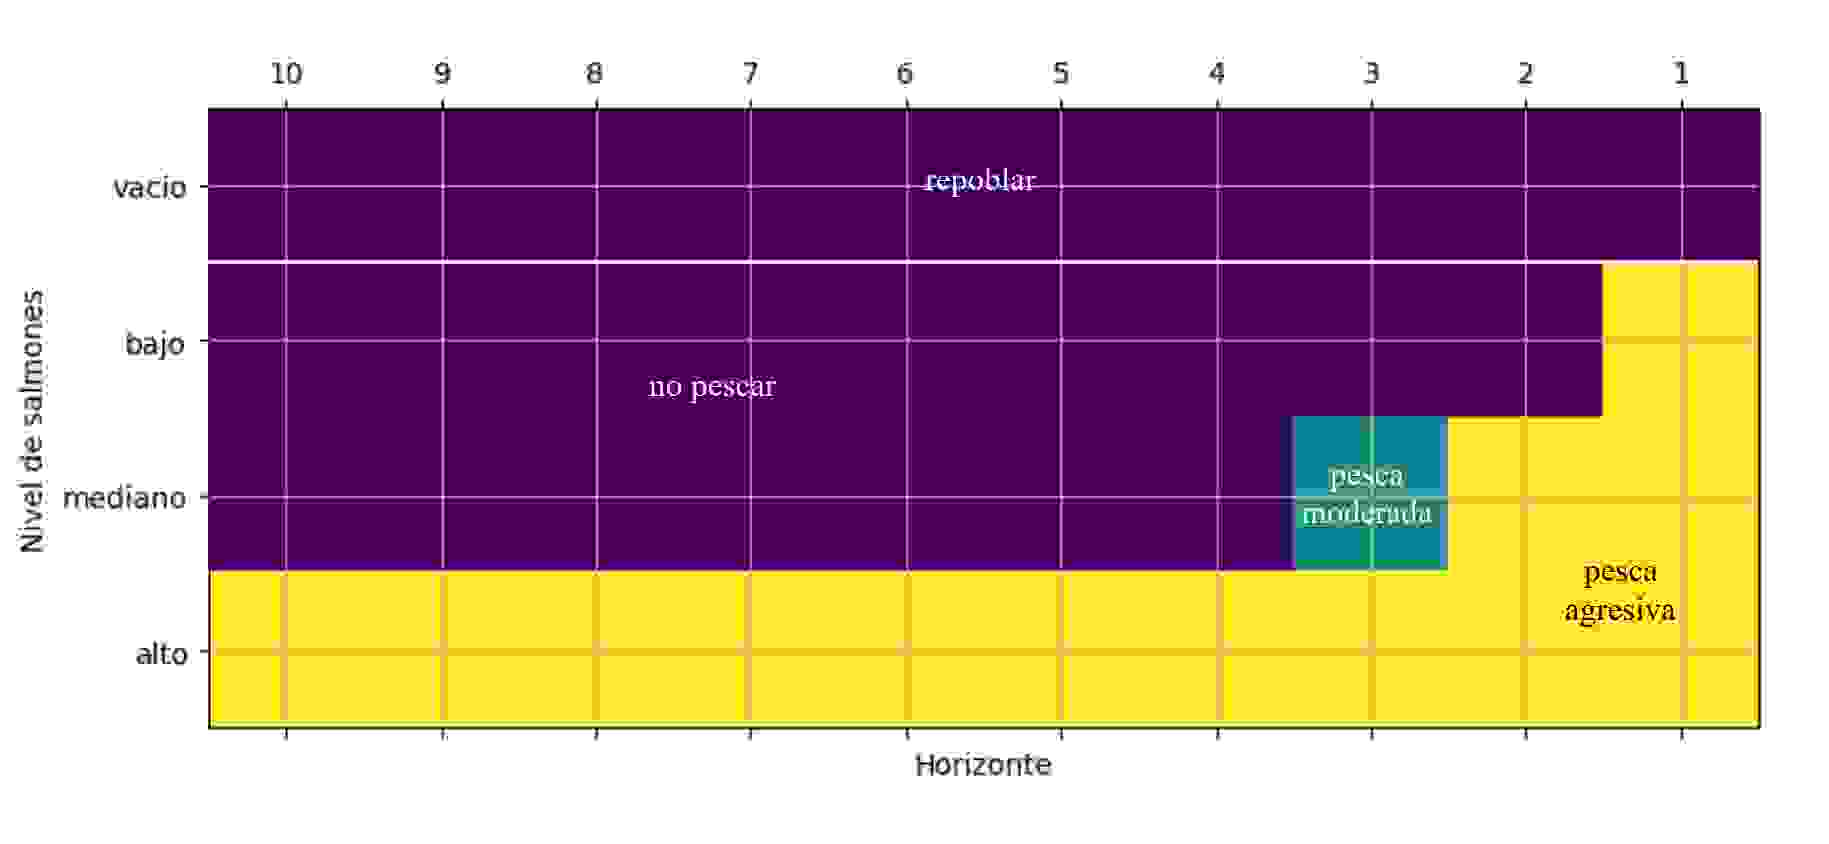
\includegraphics[width=1\textwidth]{../Images/SalmonFishing/SalmonFishingPolicy1.jpg}}}
\only<2>{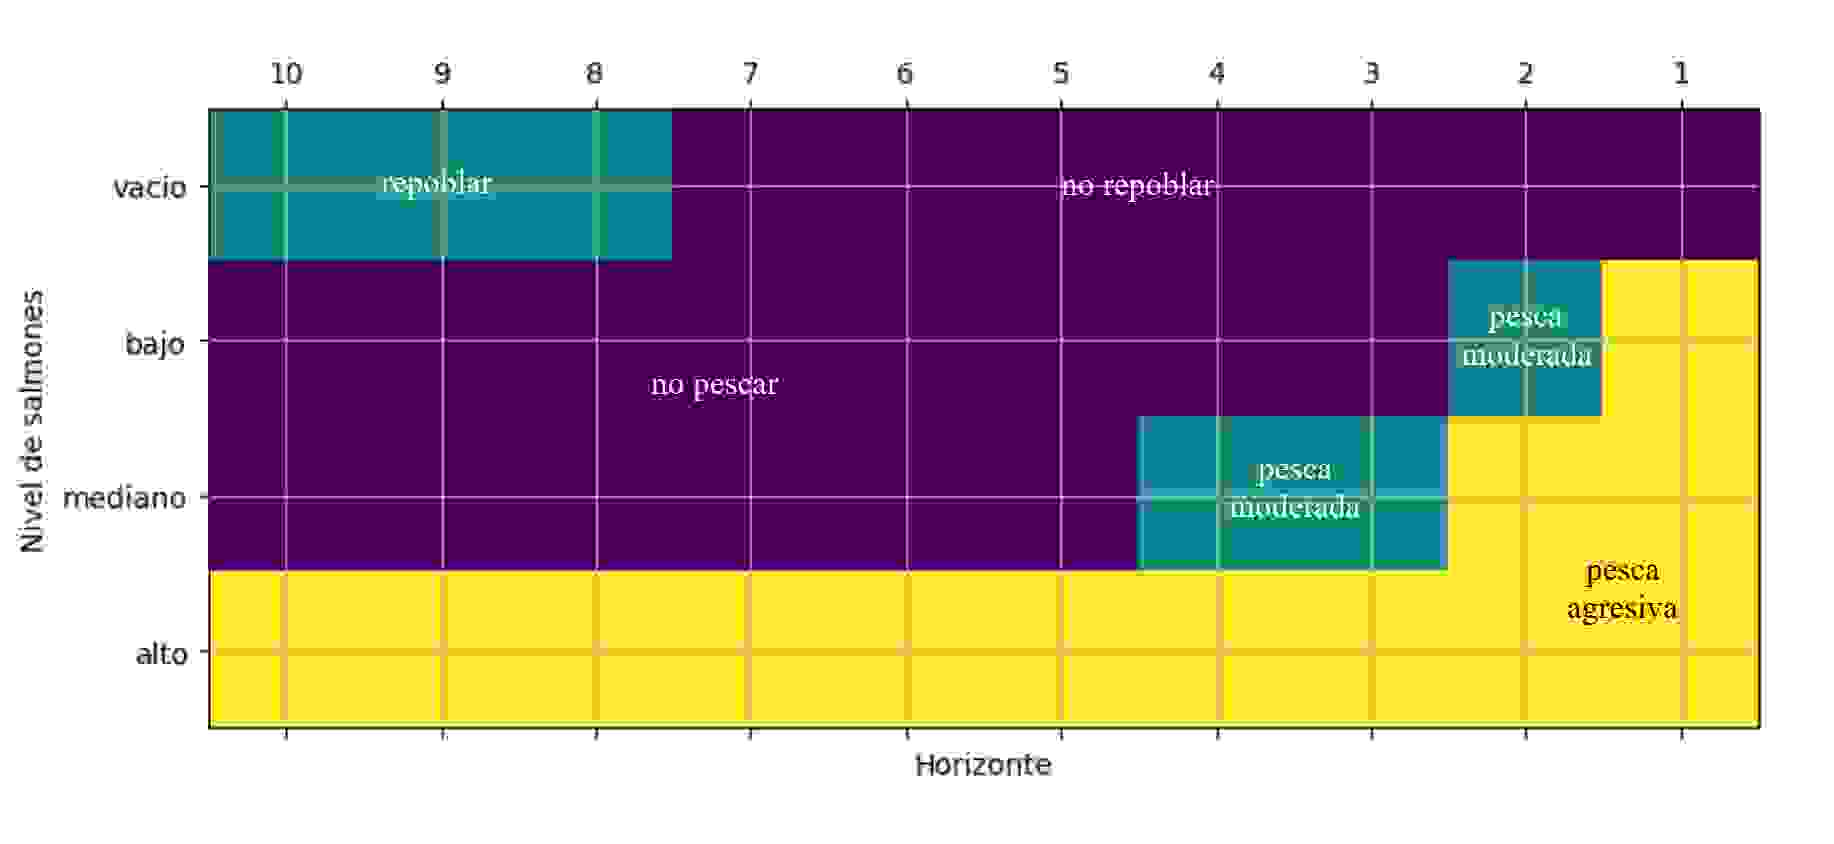
\includegraphics[width=1\textwidth]{../Images/SalmonFishing/SalmonFishingPolicy2.jpg}}
\end{center}
\end{frame}

% --- SLIDE: HORIZONTE ---
\begin{frame}{Pesca de Salmones: El Rol del Horizonte}
\begin{itemize}
    \item Para obtener la pol\'itica \'optima, debemos especificar el horizonte $T$.
    \begin{itemize}
        \item<2-> La acci\'on \'optima var\'ia seg\'un la distancia al horizonte final.
        \item<3-> \textquestiondown Qu\'e horizonte debemos elegir en la vida real?
        \item<4-> A veces la elecci\'on es natural:
        \begin{itemize}
            \item Subastas o campa\~nas electorales.
            \item Log\'istica y operaciones con fecha cr\'itica.
            \item Pricing de pasajes a\'ereos.
        \end{itemize}
    \end{itemize}
    \item<5-> \textquestiondown Qu\'e hacer si no hay un final claro para el proceso?
    \item<6-> Podemos extender el modelo hacia un \textbf{horizonte infinito}.
\end{itemize}
\end{frame}


% --- SLIDE: FORMULACIÓN INFINITA ---
\begin{frame}{MDPs con Horizonte Infinito}
Buscamos maximizar la ganancia esperada acumulada considerando un \textbf{factor de descuento} $\alpha \in [0, 1)$:
\[ V^*(s) = \max_u \mathbb{E} \left[ \sum_{t=0}^\infty \alpha^t r_{u_t}(x_t) \bigg| x_0 = s \right] \]

\begin{itemize}
    \item<2-> \textbf{Convergencia:} El factor de descuento $\alpha$ garantiza que la suma sea finita, incluso si el proceso nunca termina.
    \item<3-> \textbf{Funci\'on de Valor:}  A diferencia del horizonte finito, aqu\'i la funci\'on de valor \'optima depende solo del estado $x$, no del tiempo: $V^*(x)$.
    \item<4-> \textbf{Pol\'itica Estacionaria:} La decisi\'on \'optima tambi\'en depende solo del estado $x$: $u^*(x)$.
\end{itemize}
\end{frame}

% --- SLIDE: INTUICIÓN DEL FACTOR DE DESCUENTO ---
\begin{frame}{Factor de Descuento ($\alpha$)}
¿Por qu\'e descontar el futuro? El par\'ametro $\alpha$ captura tres conceptos clave:

\begin{enumerate}
    \item<2-> \textbf{Preferencia Temporal:} Un d\'olar hoy vale m\'as que un d\'olar ma\~nana (costo de oportunidad/inter\'es).
    \item<3-> \textbf{Incertidumbre (Supervivencia):} Podemos interpretar $(1-\alpha)$ como la probabilidad de que el proceso termine en cada paso (ej. que la empresa quiebre o el salm\'on se extinga).
    \item<4-> \textbf{Horizonte Efectivo:} Aunque el horizonte es infinito, el agente solo mira hacia el futuro una distancia aproximada de $1/(1-\alpha)$ pasos.
\end{enumerate}

\vspace{0.3cm}
\begin{exampleblock}{Comportamiento del Agente}<5->
    \begin{itemize}
        \item $\alpha \to 1$ (\textbf{Paciente}): Decisiones basadas en sostenibilidad a largo plazo.
        \item $\alpha \to 0$ (\textbf{Miope}): Decisiones ">codiciosas"< que solo buscan el beneficio inmediato.
    \end{itemize}
\end{exampleblock}
\end{frame}

\begin{frame}{Ecuaci\'on de Bellman}
\begin{itemize}
\item Con descuento $\alpha$, la recursi\'on en horizonte finito es:
% Corregido: V_t^*(s) en lugar de V^_t*(s)
\[ V_t^*(s) = \max_{a \in A} \left\{ r_a(s) + \alpha \sum_{s'} P_a(s,s') V_{t-1}^*(s') \right\} \]
 \item<2-> ¿Qu\'e sucede cuando el tiempo restante es muy grande ($T \to \infty$)?
 \item<3-> La funci\'on valor tiende a estabilizarse: $V_t \approx V_{t+1} \approx V^*$.
\end{itemize}
\only<4->{
\begin{block}{Ecuaci\'on de Bellman con Horizonte Infinito}
\[ V^*(s) = \max_{a \in A} \left\{ r_a(s) + \alpha \sum_{s'} P_a(s,s') V^*(s') \right\} \]
\end{block}}

\begin{itemize}
\item<5-> \textquestiondown C\'omo resolver la ecuaci\'on de Bellman?
\end{itemize}

\end{frame}

\begin{frame}{Iteración de Valor (VI)}
La iteraci\'on de valor toma el algoritmo recursivo de programación dinámica para horizonte finito y lo extiende a $T = \infty$. Solo se agrega un criterio de parada, basado en la convergencia de $V*$
\only<2->{
\begin{block}{Algoritmo VI}
\begin{enumerate}
    \item Inicializamos $V_0(s) = 0$ para todo $s$. (Tambi\'en funciona con otros valores iniciales.)
    \item \textbf{Actualización:} $V_{k+1}(s) \leftarrow \max_a \{ r_a(s) + \alpha \sum P V_k \}$.
    \item \textbf{Parada:} Si el cambio máximo es insignificante ($|V_{k+1} - V_k| < \epsilon$), terminamos.
\end{enumerate}
\end{block}}
\end{frame}
\begin{frame}{¿Y si nos enfocamos en la Política?}

Hasta ahora hemos iterado sobre la función de valor:

\[
V_0 \rightarrow V_1 \rightarrow V_2 \rightarrow \cdots \rightarrow V^*
\]

\vspace{0.3cm}

Pero el objetivo final no es conocer $V^*$.

\vspace{0.2cm}

\begin{center}
\Large
Queremos encontrar la política óptima $u^*$.
\end{center}

\vspace{0.3cm}

\only<2->{
\begin{alertblock}{Pregunta}
¿Podemos diseñar un algoritmo que trabaje directamente sobre políticas en lugar de funciones de valor?
\end{alertblock}
}

\end{frame}


% --- SLIDE 2: EL CICLO ACTOR-CRÍTICO ---
\begin{frame}{El Ciclo de Mejora: Actor-Cr\'itico}
Consideramos un bucle de retroalimentaci\'on fundamental en RL:

\begin{center}
\begin{tikzpicture}[
    node distance=4cm, 
    every node/.style={draw, thick, rounded corners, inner sep=8pt, font=\small, align=center},
    arrow/.style={-stealth, ultra thick}
]
  \node (politica) [fill=blue!10] {\textbf{ACTOR} \\ (Pol\'itica $u$)};
  \node (valor) [right of=politica, fill=green!10] {\textbf{CR\'ITICO} \\ (Valor $V^u$)};
  
  \draw [arrow, bend left=40] (politica) to node[above, draw=none, fill=none] {\textbf{Evaluaci\'on}: Resuelve sistema lineal} (valor);
  \draw [arrow, bend left=40] (valor) to node[below, draw=none, fill=none] {\textbf{Mejora}: Pol\'itica \textit{Greedy}} (politica);
\end{tikzpicture} 
\end{center}

\begin{itemize}
    \item<2-> \textbf{Resultado Fundamental:} Si $u'$ es la pol\'itica codiciosa con respecto a $V^u$, entonces la nueva pol\'itica es garantizadamente globalmente mejor o igual:
    \[ \mathbf{V^{u'} \geq V^u} \]
    \item<3-> \textbf{Convergencia:} Hay n\'umero finito de pol\'iticas, por ende este ciclo \textbf{debe} terminar en la pol\'itica \'optima $u^*$ en un n\'umero finito de pasos.
\end{itemize}
\end{frame}
% --- SLIDE: ALGORITMO PI ---
\begin{frame}{Iteraci\'on de Pol\'itica (PI)}
\begin{block}{Algoritmo de Iteraci\'on de Pol\'itica}
\small % Reduce ligeramente el tamaño de la fuente para ganar espacio
\begin{enumerate}
    \setlength{\itemsep}{0.5em} % Ajusta el espacio entre pasos
    \item \textbf{Inicializaci\'on ($k=0$):} Elegir una pol\'itica arbitraria $u_0(s)$.
    \item \textbf{Evaluaci\'on:} Calcular $V^{u_k}$ resolviendo el sistema:
    \[ V^{u_k}(s) = r_{u_k}(s) + \alpha \sum_{s' \in S} P_{u_k}(s, s') V^{u_k}(s') \]
    \item \textbf{Mejora:} Encontrar una pol\'itica \textit{greedy} $u_{k+1}$ respecto a $V^{u_k}$:
    \[ u_{k+1}(s) = \arg\max_{a \in A} \left\{ r_a(s) + \alpha \sum_{s' \in S} P_a(s, s') V^{u_k}(s') \right\} \]
    \item \textbf{Parada:} Si $u_{k+1} = u_k$, terminar. Si no, $k \leftarrow k+1$ y volver al paso 2.
\end{enumerate}
\end{block}
\end{frame}



%% --- SLIDE: ROLLOUT ---
%\begin{frame}{Pol\'iticas de Rollout}
%\textbf{Idea central:} Para cualquier pol\'itica $u$, una versi\'on \textit{greedy} respecto a $V^u$ garantiza una mejora (o igualdad): $V^{u'} \ge V^u$.
%
%\vspace{0.3cm}
%Este principio permite refinar heur\'isticas existentes sin ejecutar un algoritmo de optimizaci\'on completo:
%
%\begin{itemize}
%    \item \textbf{Definici\'on:} Una pol\'itica de \textit{Rollout} es el resultado de aplicar \textbf{un solo paso de mejora} a partir de una pol\'itica base $u$.
%    \item<2-> \textbf{Ventaja:} Es una forma pr\'actica y segura de "potenciar" reglas de negocio predefinidas.
%\end{itemize}
%
%\begin{block}{Aplicaciones Reales}<3->
%    \begin{itemize}
%        \item \textbf{AlphaGo:} Usa redes neuronales como pol\'itica base y \textit{rollout} (MCTS) para la toma de decisiones final.
%        \item \textbf{Log\'istica e Inventarios:} Tomar una regla simple (ej: ``reponer stock al 20\%'') y aplicar un paso de optimizaci\'on para ajustarla a la demanda actual.
%    \end{itemize}
%\end{block}
%\end{frame}

\begin{frame}{Iteraci\'on de Valor (VI) vs. Iteraci\'on de Pol\'itica (PI)}
\begin{itemize}
    \item \textbf{Convergencia:} Como el n\'umero de pol\'iticas estacionarias es finito ($|A|^{|S|}$), la iteraci\'on de pol\'itica siempre termina en la soluci\'on exacta.

    \item<2-> \textbf{Complejidad por  iteraci\'on:} 
    \begin{itemize}
        \item \textbf{PI} es m\'as costosa (requiere resolver un sistema lineal para evaluar $V^u$).
        \item \textbf{VI} es m\'as ligera (solo requiere una pasada de maximizaci\'on).
    \end{itemize}

    \item<3-> \textbf{Velocidad de convergencia:}
    \begin{itemize}
        \item \textbf{PI} suele requerir muy pocas iteraciones para converger.
        \item \textbf{VI} puede ser muy lenta, especialmente cuando el factor de descuento $\alpha$ es cercano a 1.
    \end{itemize}

    \item<4-> \textbf{En la pr\'actica:} Aunque el peor caso para PI es exponencial en $|S|$, en problemas reales suele ser extremadamente eficiente.

    \item<5-> Ambos m\'etodos son los pilares fundamentales para el desarrollo de algoritmos de \textbf{Aprendizaje por Refuerzo (RL)}.
\end{itemize}
\end{frame}

\begin{frame}{De Iteración de Política a Rollout}

La Iteración de Política repite:

\[
u \rightarrow V^u \rightarrow u' \rightarrow V^{u'} \rightarrow \cdots
\]

hasta alcanzar la política óptima.

\vspace{0.3cm}

\only<2->{
\textbf{Pregunta:}

¿Y si realizamos \emph{un solo paso} de mejora?
}

\only<3->{
\begin{block}{Política de Rollout}
Dada una política base $u$:

\[
u
\rightarrow
V^u
\rightarrow
u'
\]

La nueva política $u'$ satisface:

\[
V^{u'} \ge V^u
\]

es decir, nunca es peor que la política original.
\end{block}
}

\only<4->{
\textbf{Interpretación:}

Tomar una heurística existente y mejorarla automáticamente utilizando un modelo del problema.
}
\end{frame}




%% --- SLIDE: DISEÑO DE LA FUNCIÓN DE RECOMPENSA ---
%\begin{frame}{Diseño de la Funci\'on de Recompensa}
%La recompensa $r(s,a)$ debe capturar el objetivo final del agente. La estructura depende directamente del dominio:
%
%\begin{itemize}
%    \item \textbf{Gesti\'on de Inventario (Ganancia neta):}
%    \only<2->{
%    \[ r(x,a) = \mathbb{E}[\gamma \min(d, x+a) - \beta a - \kappa (x+a)] \]
%    \small Donde $x$ es el stock, $a$ el pedido, $d$ la demanda, $\gamma$ el precio de venta, $\beta$ el costo de pedido y $\kappa$ el costo de almacenamiento.}
%
%    \item<3-> \textbf{Navegaci\'on (Tiempo m\'inimo):}
%    \visible<4->{
%    \[ r(s) = \begin{cases} 0 & \text{si } s = s^* \text{ (meta)} \\ -1 & \text{si } s \neq s^* \end{cases} \]
%    Al maximizar una suma de $-1$, el agente busca el camino m\'as corto.}
%
%    \item<5-> \textbf{Ajedrez (Resultado binario):}
%    \visible<6->{
%    \[ r(s) = \begin{cases} +1 & \text{si gana} \\ -1 & \text{si pierde} \\ 0 & \text{en el resto} \end{cases} \]
%    \small \textbf{Problema:} Recompensa \textit{esparsa} (solo se recibe al final del juego).}
%\end{itemize}  
%\end{frame}
%
%% --- SLIDE: MULTI-OBJETIVO Y RL ---
%\begin{frame}{Dise\~no de Recompensas: Compromisos y RL}
%\begin{itemize}
%    \item \textbf{Criterios Contrapuestos:} A menudo debemos balancear objetivos.
%    \begin{itemize}
%        \item \textbf{Energ\'ia:} E\'olica + Backup de Gas.
%        \only<2->{
%        \[ r(x, d) = \underbrace{P_{wind} \cdot \min(d, W)}_{\text{Venta E\'olica}} - \underbrace{C_{gas} \cdot G}_{\text{Costo Gas}} - \underbrace{L \cdot \max(d-W-G, 0)}_{\text{Penalidad por d\'eficit}} \]
%        }
%    \end{itemize}
%    
%    \item<3-> \textbf{Consideraciones en Reinforcement Learning (RL):}
%    \begin{itemize}
%        \item<4-> \textbf{Reward Shaping:} A\~nadir recompensas intermedias para ">guiar"< al agente (ej. en ajedrez, puntuar captura de piezas). \textit{Cuidado con las consecuencias no deseadas.}
%        \item<5-> \textbf{Recompensas Esparsas:} Si el agente solo recibe feedback al final, el aprendizaje es muy lento.
%        \item<6-> \textbf{Inverse RL:} Aprender la funci\'on de recompensa observando a un experto humano.
%        \begin{itemize}
%            \item<7-> \textbf{Lecci\'on de AlphaGo:} A veces el humano es sub\'optimo porque su ">funci\'on de recompensa interna"< es limitada.
%        \end{itemize}
%    \end{itemize}
%\end{itemize}
%\end{frame}

\begin{frame}{Un Mismo Lenguaje para Problemas Distintos}

Hemos aplicado toma de decisiones secuenciales a problemas muy diferentes:

\begin{itemize}
\item Precios dinámicos en aerolíneas.
\item Gestión de recursos naturales.
\item Inventarios y logística.
\end{itemize}

\vspace{0.3cm}

Aunque los contextos son distintos, todos comparten la misma estructura:

\begin{center}
\textbf{Estado + Decisión + Incertidumbre + Consecuencias Futuras}
\end{center}

\vspace{0.3cm}

Veamos ahora una nueva aplicación: la gestión de portafolios de inversión.

\end{frame}



% --- SLIDE 1: EL PROBLEMA ---
\begin{frame}{Aplicaci\'on: Gesti\'on de Portafolios}
Imagina que debes gestionar un capital $W_t$ durante $T$ per\'iodos, eligiendo entre dos activos:
\begin{itemize}
    \item \textbf{Activo Sin Riesgo (Caja de Ahorro):} Rendimiento constante $r_f$.
    \item \textbf{Activo Con Riesgo (Acci\'on):} Precio $s_t$ que sigue un modelo \textit{lognormal}.
\end{itemize}

\begin{block}{Din\'amica del Precio (Tiempo Discreto)}
\[ s_{t+1} = s_t \cdot e^{(r - \sigma^2/2) + \sigma \epsilon_t}, \quad \epsilon_t \sim N(0,1) \]
\small Donde $r$ es el retorno esperado y $\sigma$ la volatilidad (riesgo).
\end{block}

\textbf{Objetivo inicial:} Maximizar el valor final esperado del portafolio $\mathbb{E}[W_T]$.
\end{frame}

\begin{frame}{El Modelo Lognormal: Intuici\'on}
En lugar de la f\'ormula compleja del precio, miremos el \textbf{log-rendimiento}:
\[ \xi_{t+1} = \log\left(\frac{s_{t+1}}{s_t}\right) \approx \text{Rendimiento en el periodo } t \]

\begin{itemize}
    \item \textbf{Normalidad de Rendimientos:} $\xi_t \sim N(\mu, \sigma^2)$
    
    \item<2-> \textbf{Precios No Negativos:}   $s_{t+1} = s_t \cdot e^{\xi_{t+1}}  \geq 0$

    \item<3-> \textbf{Inter\'es Compuesto:} La forma exponencial captura naturalmente que los rendimientos se reinvierten y multiplican, en vez de sumarse. 
\end{itemize}

\begin{block}{El Modelo Lognormal Completo}<4->
\[ s_{t+1} = s_t e^{ (r - \sigma^2/2) + \sigma  \epsilon_t}  \]
\small El t\'ermino $-\sigma^2/2$ es un ajuste t\'ecnico para que el valor esperado del precio crezca exactamente a tasa $r$. $\epsilon_t\sim N(0,1)~t=0,1,\dots$ son variables normales est\'andar independientes.
\end{block}
\end{frame}

\begin{frame}{De Datos Anuales a Decisiones Mensuales}

Los parámetros financieros suelen reportarse en términos anuales.

\vspace{0.2cm}

Si tomamos decisiones cada $\Delta$ años, debemos ajustar:

\begin{itemize}
\item Retorno esperado: $r_{\Delta}=r\Delta$
\item Volatilidad: $\sigma_{\Delta}=\sigma\sqrt{\Delta}$
\end{itemize}

\begin{exampleblock}{Ejemplo}
Activo con: $r=10\%, \qquad \sigma=40\%$

Si rebalanceamos mensualmente ($\Delta=1/12$):
\[
r_{mes}\approx 0.83\%,~\sigma_{mes}\approx 11.6\%
\]
\[ s_{t+1} = s_te^{ 0.001572 +0.116 \epsilon_t},~ \epsilon_t\sim N(0,1) \]

\end{exampleblock}

\end{frame}


% --- SLIDE 2: MODELADO MDP ---
\begin{frame}{Portafolio como un MDP $(S, A, P, R)$}
\begin{itemize}
    \item \textbf{Estado ($W_t$):} Riqueza total en el momento $t$.
    \item \textbf{Acci\'on ($\beta_t$):} Fracci\'on del capital invertida en el activo con riesgo ($\beta_t \in [0,1]$).
    \item \textbf{Transici\'on:} 
    \[ W_{t+1} = W_t \left[ \beta_t \underbrace{e^{(r - \sigma^2/2) + \sigma \epsilon_t}}_{\text{Retorno Acci\'on}} + (1 - \beta_t) \underbrace{e^{r_f}}_{\text{Retorno Seguro}} \right] \]
    \item \textbf{Recompensa Final:} $V_T(w) = w$. No hay recompensas intermedias.
\end{itemize}
\end{frame}


\begin{frame}{Optimización de Portafolio: Solución}
\begin{itemize}
\item Con el modelo lognormal para precios, se puede resolver la ecuaci\'on de Bellman anal\'iticamente. Tenemos:
$$
V_t^*(w) = w \max(e^r, e^{r_f})^{T-t}.
$$
\item<4-> Entonces, la política óptima no depende del tiempo ni del valor del portafolio: 
$$
\beta_{t}^*(w) = \beta* = \begin{cases}
1 & {\rm si~} r>r_f \\
0 & {\rm si~} r<r_f \\
{\rm cualquier~valor} &{\rm si~}r=r_f
\end{cases}
$$
\end{itemize}
\end{frame}

\begin{frame}{Optimización de Portafolio: Observaciones}
\begin{itemize}
\item En ese ejemplo, la solución es simple e intuitiva, reduciéndose a maximizar el rendimiento esperado en cada período. 
\begin{itemize}
\item<2-> Eso se debe a que el rendimiento del activo es independiente y distribuido igualmente a cada periodo.
\end{itemize}
\item<3-> La metodología puede ser aplicada en condiciones más complejas, por ejemplo:
\begin{itemize} 
\item<4-> la tasa de interés, el rendimiendo de la acción y su volatilidadd pueden ser fluctuantes;
\item<5-> pueden haber costos para realizar transacciones.
\end{itemize}
\item<6-> En este caso tanto la variable de estado como la acción son contínuas.
\begin{itemize}
\item<7-> \textquestiondown Qu\'e hacer si una solución analítica no existe? \only<8->{Necesitamos realizar aproximaciones, por ejemplo discretizando el espacio de estados y/o el espacio de acciones.}
\end{itemize}
\end{itemize}
\end{frame}

% --- SLIDE 3: SOLUCIÓN Y RESULTADO ---
\begin{frame}{Soluci\'on por Inducci\'on Hacia Atr\'as}
Al resolver la ecuaci\'on de Bellman $V_t^*(w) = \max_{\beta} \mathbb{E}[V_{t+1}^*(W_{t+1})]$, encontramos un resultado sorprendente:

\begin{itemize}
    \item \textbf{Pol\'itica Óptima:} 
    \[ \beta^* = \begin{cases} 1 & \text{si } r > r_f \\ 0 & \text{si } r < r_f \end{cases} \]
\end{itemize}

\begin{alertblock}{Conclusi\'on "Peligrosa"}
    El agente decide invertir \textbf{todo} o \textbf{nada} en el activo de riesgo. No diversifica. 
    \textit{¿Por qu\'e sucede esto?} Porque maximizar el valor esperado ignora por completo el \textbf{riesgo} (volatilidad).
\end{alertblock}
\end{frame}

\begin{frame}{Distribuci\'on del Rendimiento Seg\'un la Volatilidad}
\begin{itemize}
\item<1-> $R_{\rm riesgo} = e^{r-\sigma^2/2+\sigma \epsilon}$, , donde $\epsilon \sim {\rm N}(0,1)$, y $R_{\rm ahorro} = e^{r_f}$
\item<2-> Generamos la distribución de $R_{\rm riesgo}$ con Python...
\visible<3->{
\begin{center}
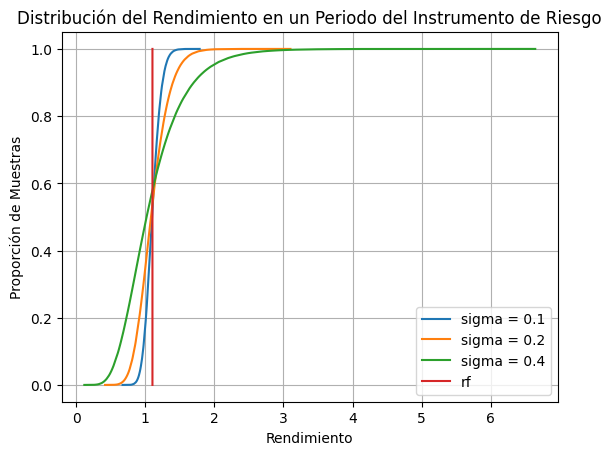
\includegraphics[width=0.8\textwidth]{../Images/Portfolios/StockReturns.png}
\end{center}}
\item<4-> Somos indiferentes a esas cuatros opciones?
\end{itemize}
\end{frame}
% --- SLIDE: DISEÑO DE RECOMPENSA Y AVERSIÓN AL RIESGO ---
\begin{frame}{Diseño de Recompensa: Aversi\'on al Riesgo}
Maximizar el valor esperado $\mathbb{E}[W_T]$ ignora la volatilidad, resultando en decisiones de "todo o nada". Para capturar el comportamiento humano real, debemos repensar la recompensa.

\begin{exampleblock}{El Dilema de la Moneda}
    ¿Qu\'e preferir\'ias recibir?
    \begin{itemize}
        \item \textbf{Opci\'on A:} US\$500,000 garantizados (seguridad).
        \item \textbf{Opci\'on B:} Una moneda al aire por US\$0 o US\$1,000,000 (riesgo).
    \end{itemize}
    \textit{Aunque el valor esperado es el mismo (US\$500k), la mayor\'ia elige la seguridad. Esto es la \textbf{Aversi\'on al Riesgo}.}
\end{exampleblock}

\only<2-.>
{Perder US\$500000 duele m\'as que ganar US\$500000. \textquestiondown C\'omo capturamos esa preferencia?}
\only<3->{Mediante las \textbf{funciones de utilidad}.}
\end{frame}

\begin{frame}{Funciones de Utilidad}
Para representar la postura ante el riesgo, no maximizamos el valor nominal, sino la \textbf{Utilidad} del dinero: $\max \mathbb{E}[u(W_T)]$.

\begin{itemize}
    \item<2-> \textbf{Aversi\'on al riesgo ($u(w)$ c\'oncava):} Preferimos un resultado seguro a una apuesta con el mismo valor esperado.
    \item<3-> \textbf{Neutralidad al riesgo ($u(w)$ lineal):} Solo nos importa el valor esperado; es el caso que vimos al inicio.
    \item<4-> \textbf{Preferencia por el riesgo ($u(w)$ c\'onvexa):} Se valora la posibilidad de grandes ganancias por encima de la estabilidad.
\end{itemize}



\visible<5->{
\begin{center}
    \textit{En econom\'ia y finanzas, la norma es la \textbf{concavidad}: el "dolor" de perder \$1 es mayor que el "placer" de ganar \$1.}
\end{center}}
\end{frame}

% --- SLIDE: UTILIDAD CRRA ---
\begin{frame}{Utilidad CRRA: Aversi\'on Relativa Constante}
La funci\'on m\'as utilizada es la \textbf{CRRA} (\textit{Constant Relative Risk Aversion}):
\[ u(w) = \frac{w^\gamma}{\gamma}, \quad \text{con } \gamma < 1, \, \gamma \neq 0 \]

\begin{itemize}
    \item \textbf{¿Qu\'e significa "Relativa Constante"?} 
    Tu tolerancia al riesgo es \textbf{proporcional} a tu riqueza. La fracci\'on de capital invertida en riesgo ($\beta$) no cambia si tu riqueza aumenta de \$1,000 a \$1M.
    
    \item<2-> \textbf{El papel de $\gamma$ (Par\'ametro de riesgo):}
    \begin{itemize}
        \item $\gamma \to 1$: Neutral al riesgo (se vuelve lineal).
        \item $\gamma \to 0$: Converge a \textbf{$u(w) = \log(w)$}.
        \item $\gamma < 0$: El agente es altamente conservador (aversi\'on extrema).
    \end{itemize}
\end{itemize}
\end{frame}

\begin{frame}{Visualizando la Funci\'on de Utilidad}
\begin{center}
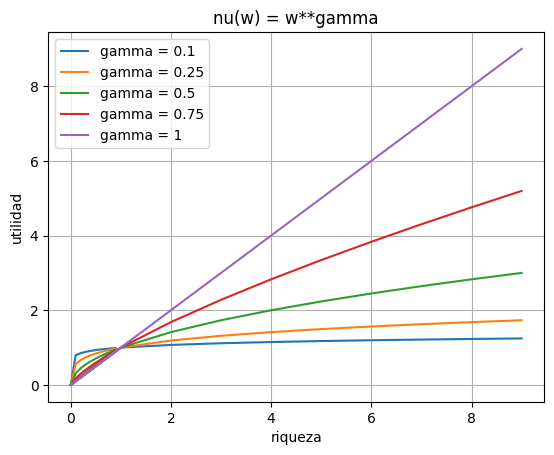
\includegraphics[width=0.5\textwidth]{../Images/Portfolios/UtilityFunction2.png}    
\end{center}

\begin{block}{Intuici\'on de la Curvatura}<3->
    Cuanto menor es $\gamma$, m\'as ">curvada"< es la funci\'on. Esto penaliza fuertemente los resultados bajos, obligando al MDP a elegir una fracci\'on de riesgo $\beta$ m\'as pequeña.
\end{block}
\end{frame}

% --- SLIDE 3: PORTAFOLIO CON UTILIDAD ---
\begin{frame}{Optimizaci\'on con Utilidad (CRRA)}
Al introducir $u(w) = w^\gamma$, la ecuaci\'on de Bellman cambia. La nueva pol\'itica \'optima $\beta^*$ ahora \textbf{s\'i considera la volatilidad}:

\[ \beta^*_\gamma = \arg\max_{\beta \in [0,1]} \mathbb{E} \left[ \left( \beta e^{r-\sigma^2/2+\sigma \epsilon} + (1-\beta)e^{r_f} \right)^\gamma \right] \]

\begin{itemize}
    \item<2-> Ya no es "todo o nada". El agente diversifica.
    \item<3->  Sin embargo, con esta funci\'on (CRRA), la fracci\'on $\beta^*$ no depende de cu\'anta plata ten\'es ($w$), lo cual simplifica mucho la gesti\'on.
\end{itemize}
\end{frame}

\begin{frame}{¿Cuándo Depende la Política del Estado?}

En nuestro modelo con utilidad CRRA, vimos que $\beta^*$ es una constante. La fracción óptima invertida no depende de la riqueza $w$.

\vspace{0.3cm}

\only<3->{
\textquestiondown Cu\'ando la política depende del estado? Cuando éste afecta:

\begin{itemize}
\item \textbf{Las acciones disponibles}
\begin{itemize}
\item Límites de endeudamiento.
\item Requerimientos mínimos de efectivo.
\item Costos de transacción.
\end{itemize}

\item \textbf{Las oportunidades futuras}
\begin{itemize}
    \item Regímenes de mercado (bull/bear).
    \item Horizonte restante hasta el objetivo.
    \item Ingresos futuros esperados.
\end{itemize}

\end{itemize}
}

\end{frame}


%% --- SLIDE 4: EL MODELO COMPLETO (CONSUMO) ---
%\begin{frame}{MDP Completo: Inversi\'on y Consumo}
%En la vida real, no solo invertimos, tambi\'en gastamos.
%\begin{block}{Modelo de Merton simplificado}
%\begin{itemize}
%    \item \textbf{Estado:} Riqueza actual $W_t$.
%    \item \textbf{Acciones:} 
%        \begin{enumerate}
%            \item $\delta_t$: Qu\'e fracci\'on de mi riqueza \textbf{consumo} hoy.
%            \item $\beta_t$: Qu\'e fracci\'on de lo que sobra \textbf{invierto} en riesgo.
%        \end{enumerate}
%    \item \textbf{Recompensa:} Utilidad del consumo presente $u(\delta_t W_t)$.
%\end{itemize}
%\end{block}
%
%\visible<2->{
%\[ V^*(w) = \max_{\beta, \delta} \left\{ u(\delta w) + \alpha \mathbb{E} [ V^*(W_{t+1}) ] \right\} \]
%\small El agente ahora balancea: \textbf{Vivir bien hoy} vs. \textbf{Invertir para vivir bien ma\~nana}.
%}
%\end{frame}

\begin{frame}{Los Límites de MDPs}

Los MDPs nos permiten formular problemas de decisión secuencial y encontrar políticas óptimas. Pero los métodos exactos que hemos estudiado enfrentan dos desafíos importantes:

\begin{enumerate}
\item<2-> \textbf{Modelo desconocido}

Las probabilidades de transición y recompensas pueden no estar disponibles. Deben aprendera actuar \'optimamente a partir de datos o experiencia.

\item<3-> \textbf{Espacios de estados enormes}

Incluso conociendo el modelo, almacenar y calcular $V(s)$ para todos los estados puede ser imposible, cuando el espacio de estados es demasiado grande.

\end{enumerate}

\only<4->{
\begin{alertblock}{La Idea del RL}
Aprender y mejorar políticas a partir de simulación o experiencia, sin depender de modelos exactos ni de recorrer exhaustivamente todos los estados.
\end{alertblock}
}

\end{frame}


%% --- SLIDE: REFLEXIÓN FINAL ---
%\begin{frame}{¿Es todo una suma de recompensas?}
%Hemos trabajado bajo la \textit{Hipótesis de la Recompensa}: la idea de que cualquier objetivo puede capturarse maximizando una señal escalar acumulada.
%
%\begin{itemize}
%    \item<2-> \textbf{La tiranía del escalar:} ¿Podemos realmente reducir conceptos como la \textbf{equidad}, la \textbf{curiosidad} o la \textbf{seguridad} a un solo número?
%    \item<3-> \textbf{El problema del diseño:} Si el agente encuentra un "atajo" para obtener recompensa sin cumplir el objetivo real (\textit{reward hacking}), ¿falló el algoritmo o falló nuestra definición de éxito?
%    \item<4-> \textbf{L\'imites del MDP:} ¿Existen comportamientos que simplemente no pueden expresarse como una suma de estados y acciones?
%\end{itemize}
%
%\begin{block}{El Desaf\'io}<5->
%    Hasta ahora, hemos asumido que conocemos las reglas del juego ($P$) y los premios ($r$). Pero, ¿qué sucede cuando el agente debe aprender en un mundo cuyas reglas desconoce y cuyo estado es casi infinito?
%\end{block}
%
%\vspace{0.5cm}
%\visible<6->{\centering \textit{\textbf{Continuar\'a...}}}
%\end{frame}
\end{document}